%%	Dokument-Wrapper nach der Vorlage von Herrn Plate.

%% Standard-Vorspann
\documentclass[a4paper,12pt,oneside]{report}
\usepackage[english,ngerman]{babel}                   
\usepackage[utf8]{inputenc}
\usepackage[T1]{fontenc}
\usepackage[fleqn]{amsmath}


%% Auf Schriftart Palatino umschalten
\usepackage{mathpazo}
\usepackage[scaled=.95]{helvet}
\usepackage{courier}

%% fast immer benoetigte Pakete
\usepackage{epsfig}
\usepackage{amssymb}
\usepackage{alltt}
\usepackage{latexsym}
\usepackage{makeidx}
\usepackage{textcomp}
\usepackage{rotating}
\usepackage{color}
\usepackage{caption}
\usepackage{verbatim}
\usepackage{fancyhdr}
\usepackage[printonlyused]{acronym}
\usepackage[hyperfootnotes=false ,hidelinks, linktoc=all]{hyperref}


%% spezielles Zeug
\usepackage[tablename=Tbl.]{caption}
\usepackage{nomencl}
\usepackage[subfigure]{tocloft}
\usepackage{Abschlussarbeit}
\usepackage{geometry}
\usepackage{graphicx}
\usepackage[onehalfspacing]{setspace}
\usepackage{bibgerm}
\usepackage{footnote}
\usepackage[bottom]{footmisc}
\usepackage{longtable}
\usepackage{multirow}
\usepackage{wrapfig}
\usepackage{subfigure}
\usepackage{float}

\graphicspath{{graphics/}}
\geometry{left = 4cm, right = 2cm, top = 2cm, bottom = 2cm}

\captionsetup[table]{labelfont=bf,textfont=it}
\captionsetup[figure]{labelfont=bf,textfont=it}
\captionsetup{format=hang,indention=0pt,justification=raggedright, singlelinecheck=false}
\addto\captionsngerman{\renewcommand{\figurename}{Abb.}}

\renewcommand{\nomname}{Abkürzungsverzeichnis}

\setlength{\cftfignumwidth}{3em}

%% Neue umgebung definieren für 2 Abstracts auf einer Seite ohne \clearpage
\newenvironment{abstractDuo}{
	\begin{center}%
		\bfseries\abstractname
	\end{center}}%

%\makenomenclature


%% Index erzeugen
\makeindex

%% jetzt geht's los
\begin{document}
	\raggedbottom
	
	%% Die Datei "Vorspann.tex"  bitte ausfüllen!
	\pagenumbering{Roman}
\begin{titlepage}
	\begin{figure}[h]
		 
		\begin{minipage}{0.45\linewidth} 
			\raggedright 
			
\includegraphics[scale=0.15]{HMLogo.png} 
		\end{minipage} 
		\begin{minipage}{0.45\linewidth} 
			\raggedleft
			\vspace*{1 cm} 
			
\includegraphics[scale=0.4]{sielogopetrolcmyk.jpg} 
		\end{minipage} 
	\end{figure}
	\begin{center} 
		\vspace{1.5 cm} {\LARGE Hochschule München} \\ 
		\vspace{1 cm} {\LARGE Fakultät für Elektrotechnik und Informationstechnik} \\ 
		\vspace{2 cm} {\Large Studiengang Elektrotechnik und Informationstechnik} \\ 
		\vspace*{2 cm}{\Huge \bf Industrie 4.0 - Pathfinding auf einer SPS\\} 
		\vspace{2 cm}
		{\bf Bachelorarbeit von Niels Garibaldi}\\
	\end{center}
	\vspace{4 cm}
	\begin{center}
		
		\begin{tabular}{ll}
			
			{\bf Bearbeitungsbeginn:} & xx.xx.2016\\
			{\bf Abgabetermin:} & xx.xx.2016\\
			{\bf lfd. Nr.:} & xxxxx\\
		\end{tabular}
	\end{center}

\end{titlepage} 

\begin{titlepage}
	\begin{figure}[h]
		
		\begin{minipage}{0.45\linewidth} 
			\raggedright 
			
\includegraphics[scale=0.15]{HMLogo.png} 
		\end{minipage} 
		\begin{minipage}{0.45\linewidth} 
			\raggedleft
			\vspace*{1 cm} 
			
\includegraphics[scale=0.4]{sielogopetrolcmyk.jpg} 
		\end{minipage} 
	\end{figure}
	\begin{center} 
		\vspace{1.5 cm} {\LARGE Hochschule München} \\ 
		\vspace{1 cm} {\LARGE Fakultät für Elektrotechnik und Informationstechnik} \\ 
		\vspace{2 cm} {\Large Studiengang Elektrotechnik und Informationstechnik} \\ 
		\vspace*{2 cm}{\Huge \bf Industrie 4.0 - Pathfinding auf einer SPS\\} 
		\vspace{1 cm}
		\hrule
		\vspace*{1 cm}{\Huge \bf Industry 4.0 - Pathfinding on a PLC\\} 
		\vspace{2 cm}
		{\bf Bachelorarbeit von Niels Garibaldi}\\
		\vspace{1 cm}
		{\bf betreut von  Prof. Dr. K. Ressel}\\
		
	\end{center}
	\vspace{1 cm}
	\begin{center}
		
		\begin{tabular}{ll}
			
			{\bf Bearbeitungsbeginn:} & xx.xx.2016\\
			{\bf Abgabetermin:} & xx.xx.2016\\
			{\bf lfd. Nr.:} & xxxxx\\
		\end{tabular}
	\end{center}
	
\end{titlepage}
\pagestyle{headings}
\clearpage
\phantomsection
\addcontentsline{toc}{section}{Erklärung des Bearbeiters}
\section*{Erklärung des Bearbeiters}



\begin{enumerate}
	\vspace{2 cm}
	\item
		Ich erkläre hiermit, dass ich die vorliegende Bachelorarbeit selbständig
		verfasst und noch nicht anderweitig zu Prüfungszwecken vorgelegt habe.\\
		
		Sämtliche benutzte Quellen und Hilfsmittel sind angegeben, wörtliche
		und sinngemäße Zitate sind als solche gekennzeichnet.\\
	
	\item
		Ich erkläre mein Einverständnis, dass die von mir erstellte Bachelorarbeit in die Bibliothek
		der Hochschule München eingestellt wird. Ich wurde darauf hingewiesen, dass die
		Hochschule in keiner Weise für die missbräuchliche Verwendung von Inhalten durch Dritte
		infolge der Lektüre der Arbeit haftet. Insbesondere ist mir bewusst, dass ich für die
		Anmeldung von Patenten, Warenzeichen oder Geschmacksmustern selbst verantwortlich
		bin und daraus resultierende Ansprüche selbst verfolgen muss. 
	
	\vspace{6 cm}
\end{enumerate}
\begin{flushright}
	\begin{tabular}{cl}
		München, den xx.xx.2016, & \_\_\_\_\_\_\_\_\_\_\_\_\_\_\_\_\_\_\_\_\_\_\_\_\_\_\_\_\_\_\_\_\_\_\_\_\_\_\tabularnewline
		& Niels Garibaldi\tabularnewline
	\end{tabular}
	\par
\end{flushright}
\clearpage

%% Kurzfassung/Abstract
\phantomsection
\addcontentsline{toc}{section}{Zusammenfassung/Abstract}	
\begin{abstractDuo}
	Zusammenfassungstext hier einfügen
\end{abstractDuo}
\selectlanguage{english}
\vspace{8 cm}
\begin{abstractDuo}
	Insert abstract text here
\end{abstractDuo}
\selectlanguage{ngerman}
\clearpage
%% Inhaltsverzeichnis
\pagestyle{plain}
\clearpage
\phantomsection
\addcontentsline{toc}{section}{\contentsname}

	\begin{spacing}{1.1}
	
		\tableofcontents
	\end{spacing}
\clearpage
\addcontentsline{toc}{section}{Abkürzungsverzeichnis}	
\section*{Abkürzungsverzeichnis}
\begin{acronym}[Bash]
	
	\acro{AWL}{Anweisungsliste}
	\acro{CPS}{Cyber-physisches System}
	\acro{CPPS}{Cyber-physisches Produktionssystem}
	\acrodefplural{CPPS}{Cyber-physische Produktionssysteme}
	\acro{CT}{Corporate Technologies}
	\acro{D*}{Focussed Dynamic A*}
	\acro{DB}{Datenbaustein}
	\acro{FB}{Funktionsbaustein}
	\acro{FC}{Funktion}
	\acro{FTF}{Fahrerloses Transportfahrzeug}
	\acro{FTS}{Fahrerloses Transportsystem}
	\acro{FUP}{Funktionsplan}
	\acro{IoT}{Internet of Things}
	\acro{KOP}{Kontaktplan}
	\acro{MA*}{Memory Bounded A*}
	\acro{OB}{Organisationsbaustein}
	\acro{PLC}{Programmable Logic Controller}
	\acro{RTA*}{Real-Time A*}
	\acro{SCL}{Structured Control Language}
	\acro{SPS}{Speicherprogrammierbare Steuerung}
	\acrodefplural{SPS}{Speicherprogrammierbare Steuerungen}
	\acro{STEP7}{STeuerungen Einfach Programmieren Version 7}
	\acro{TCP}{Transport Control Protocol}
	\acro{TIA-Portal}{Totally Integrated Automation Portal}
	\acro{UDP}{User Datagramm Protocol}

\end{acronym}

%%Nomenclature definitions


%	\nomenclature{CPS}{Cyber-physisches System}
%	\nomenclature{CPPS}{Cyber-physisches Produktionssystem}
%	%\acrodefplural{CPPS}{Cyber-physische Produktionssysteme}
%	\nomenclature{IoT}{Internet of Things}
%	\nomenclature{PLC}{Programmable Logic Controller}
%	\nomenclature{SPS}{Speicherprogrammierbare Steuerung}




\clearpage
\pagestyle{headings}
\pagenumbering{arabic}
  
	
	%% Hier kommt der eigentlich Text der Arbeit
	%% sinnvoll ist, für jedes Kapitel eine eigene 
	%% Datei zu nehmen, verkürzt die Zeit beim LaTeX-Durchlauf
	%% Erst am Schluss alle Dateien verwenden.
	
	\chapter{Einführung in das Thema Industrie 4.0}

Der Begriff "`Industrie 4.0\index{Industrie 4.0}"' ist seit seiner Einführung durch die Bundeskanzlerin auf der Hannovermesse 2013 vor allem in den Bereichen Produktion und Fertigung in aller Munde. Da er jedoch je nach Branche unterschiedliche Bedeutungen haben kann, möchte ich als Einführung zunächst einmal erläutern, was Industrie 4.0 im Kontext der Automatisierungstechnik bedeutet.
%% Nachdem im Verlauf der vorhergehenden industriellen Revolutionen Menschliche Arbeitskraft zunächst durch Maschinen ersetzt wurde(erste industrielle Revolution), diese dann im Zuge der Massenproduktion zusammengeschaltet wurden(zweite industrielle Revolution) und dann Mitte diesen Jahrhunderts durch den Einsatz von elektrischen und informationstechnischen 
Der Begriff beschreibt die vierte industrielle Revolution und die damit einhergehende Verflechtung von informationstechnisch erhobenen Daten in den Produktionsablauf. Ein interessanter Aspekt ist hier beispielsweise der Bereich der prädiktiven Wartung, bei dem Anhand der Auswertung empirischer Daten mögliche Anlagenausfälle frühzeitig erkannt und behoben werden können.\\
Für den weiteren Verlauf dieser Arbeit ist vor allem auch ein sogenanntes \ac{CPPS} von Bedeutung. Diese bestehen aus der Verbindung von einzelnen, dezentralen Objekten wie beispielsweise Produktionsanlagen oder Logistikkomponenten, welche mit eingebetteten Systemen ausgestattet und zudem kommunikationsfähig gemacht werden. Durch eingebaute Sensoren und Aktoren kann die Umwelt erfasst und beeinflusst werden. Mittels der Kommunikationskomponenten können Daten aus der Produktion über ein Netzwerk oder das Internet ausgetauscht, beziehungsweise von entsprechenden Diensten ausgewertet, verarbeitet oder gespeichert werden.
\cite{Bauerhansl2014}\\
Sind mehrere \aclp{CPPS} an einem Produktionsprozess beteiligt, unabhängig von ihrem Standort, so spricht man auch von einer Smart Factory\index{Smart Factory}.
Abschließend ist noch zu erwähnen, dass der Begriff "`Industrie 4.0"' vor allem im deutschsprachigen Raum verwendet wird. Im internationalen Kontext werden viele der zentralen Punkte von Industrie 4.0 durch das Konzept des \ac{IoT} abgedeckt.




 
	
	\chapter{Definition der Anforderungen}

\section{Allgemeine Aufgabenstellung}

	Diese Arbeit beschäftigt sich mit dem Entwurf und der Realisierung eines \ac{CPPS} im Modellmaßstab. Die resultierende Anlage soll unter anderem dazu dienen verschiedene Aspekte von Industrie 4.0 vorzuführen und zu veranschaulichen. Kernpunkte, die dargestellt werden sollen, sind vor allem die Dezentralisierung und Skalierbarkeit der Anlage. Den Rahmen für die Bearbeitung dieser Aufgabe bildet die Fachberatung für Automatisierungstechnik der Siemens AG in München. Um die erwähnten Konzepte demonstrieren zu können, soll die Anlage gemäß ihrer realen Vorbilder bestehen aus Bearbeitungsstationen, an welchen der Bearbeitungsprozess simuliert werden kann, und Werkstückträgern, welche Werkstücke durch die Modellanlage zu den Maschinenplätzen transportieren können. Hauptaufgabe des Modells ist es zu zeigen, wie ein Werkstück seine Fertigung selbst organisiert. Zu Beginn des Fertigungsprozesses wird dem Werkstück ein Fertigungsplan übergeben, anhand welchem es sich durch die Anlage bewegt. Im vorliegenden Fall stellen die Werkstückträger gleichzeitig das Werkstück dar, dass die Produktionsanlage durchfährt. Ebenso werden die Bearbeitungsstationen nur symbolisch dargestellt durch entsprechende Markierungen in der Anlagentopologie. Anhand verschiedener Use-cases und Szenarien soll es nach Fertigstellung der Anlage möglich sein, verschiedene Aspekte von Industrie 4.0 anschaulich darzustellen, zum Beispiel zu Vorführzwecken bei Kunden.

\section{Aufteilung der Themenbereiche}

	Wie soeben beschrieben konzentriert sich die Aufgabe vor allem auf die Entwicklung und Implementierung der Werkstückträgerfahrzeuge. Da dies jedoch noch immer ein recht allgemein gefasstes Themengebiet ist und der zur Realisierung notwendige Aufwand nur schwer abzuschätzen ist, wurde in Rücksprache mit dem Betreuer entschieden, die Hauptaufgabe in zwei Teilaufgaben zu unterteilen. Diese beiden Themenblöcke sind "`Autonomes Fahren in industriellen Transportsystemen"' und "`Dynamische Wegfindung in einer flexiblen Produktionsanlage"'\cite{I40Modell}.Die Dokumentation der Implementierung der dynamischen Wegfindung ist Hauptbestandteil der vorliegenden Arbeit. Den Teil des autonomen Fahrens mittels eines \ac{FTS} wird von Herrn Andreas Meier bearbeitet und wird deshalb nur kurz umrissen.

\subsection{Fahrerloses Transportsystem}
	Hauptaufgabe der Werkstückträger, die jeweils durch ein \ac{FTF} realisiert werden sollen, ist es, einen Weg anhand einer vorgegebenen Route ab zu fahren und somit die Werkstücke zwischen den einzelnen Bearbeitungsschritten zur nächsten Station oder Maschine zu transportieren. Herausforderungen hierbei sind die Spurführung und die Navigation innerhalb der Anlagentopologie, da die einzelnen \ac{FTF} nicht wie sonst üblich schienengebunden sind, sondern sich frei durch die Anlage bewegen können. Da es sich zudem mehrere Fahrzeuge gleichzeitig in der Anlage befinden können, muss durch geeignete Sensorik eine bevorstehende Kollision erkannt und verhindert werden.
\subsection{Dynamische Wegfindung}
	Für die Wegfindung ist es wichtig, dass das Werkstück die Ablaufreihenfolge der benötigten Arbeitsschritte kennt. Diese sollen in einer Art Rezept festgehalten werden und als Grundlage für die Berechnung der Teilrouten zu den Bearbeitungsstationen dienen. Für die Bestimmung der Routen wird zudem eine geeignete Beschreibung der Anlagentopologie benötigt. Innerhalb der Anlage können mehrere Bearbeitungsstationen die gleiche Funktionalität liefern. In diesem Fall soll die Wegfindung eine geeignete Station auswählen können Diese sollte universell gehalten sein, damit sie auch von dem \ac{FTS} genutzt werden kann. Die Wegfindung soll so realisiert sein, dass sie auch auf einer der leistungsschwächeren Steuerungen der Siemens S7-1200er Reihe lauffähig ist, falls dies nicht realisierbar ist, sollen so wenig Komponenten wie möglich auf ein PC-System ausgelagert werden.
	\\ Bei der Berechnung von Routen sollen zudem folgende dynamische Ereignisse berücksichtigt werden:
	\begin{itemize}
		\item Persistente Blockaden und länger andauernde  nicht permanente Änderungen der Standard-Anlagentopologie.
		\item Dynamische Blockaden von Teilstrecken durch andere Fahrzeuge zur Kollisionsvermeidung.
	\end{itemize}
	
	

\section{Erwartete Ziele für die Wegfindung}
	Da bei der Planung des Arbeitsauftrags noch nicht absehbar war, wie zeitaufwendig die Realisierung der Aufgabe sein würde, wurde die Funktionalität der Wegfindungskomponente der Anlage in mehrere Stufen unterteilt:
	\begin{enumerate}
		\item[\textbf{Grundstufe:}] Es können detaillierte Teilrouten generiert werden auf der Basis von Anfangs- und Endpunkten.
		\item[\textbf{Stufe 1:}] Es können komplette Routen bestehend aus Teilrouten anhand eines einzigen Fertigungsplans generiert werden, es existiert pro Funktionalität nur eine Bearbeitungsstation. Mehrere \ac{FTF} erhalten die gleiche Route und reihen sich hintereinander ein.
		\item[\textbf{Stufe 2:}] Es wird werden komplette Routen anhand eines einzigen Fertigungsplans generiert, pro Funktionalität existieren mehrere Bearbeitungsstationen. Die \ac{FTF} können unterschiedliche Wege nehmen und sich gegenseitig überholen.
		\item[\textbf{Stufe 3:}] Analog zu Stufe 2, es können jedoch im laufenden Betrieb Störungen in der Form von persistenten Blockaden auftreten, die bei der Wegfindung berücksichtigt werden.
		\item[\textbf{Stufe 4:}] Analog zu Stufe 3, verschiedene Fahrzeuge können unterschiedliche Fertigungspläne und somit andere Routen verfolgen.
	\end{enumerate}
	Als zusätzliches Ziel wurde die Visualisierung der geplanten und bereits zurückgelegten Fahrstrecken der verschieden \ac{FTF} definiert, zur besseren Darstellung der einzelnen Aspekte der definierten Stufen. Die Anlage wird zudem in Kooperation mit der Siemens Entwicklungsabteilung \ac{CT} entwickelt wird, welche parallel die gleiche Anlage als Simulation testet und die ermittelten Ergebnisse mit dem Resultat der physikalischen Anlage vergleicht.
	
	
	\chapter{Theoretische Grundlagen Wegfindung}

\section{Modellierung der Anlagentopologie}
	\label{Graph_Anlage}
	Zur Berechnung eines Weges innerhalb der Anlage wird zuallererst die Topologie der besagten Anlage benötigt. Für die Funktionsweise der \ac{FTF} wurde definiert, das sich alle Fahrzeuge mittels optischer Merkmale auf einer definierten Teilstrecke bewegen. Zudem soll es den Fahrzeugen nur an festgelegten Entscheidungspunkten möglich sein, ihren Fahrzustand zu ändern und eine andere Teilstrecke. Dies bedeutet, das alle Fahrzeuge, sobald sie sich für eine Teilstrecke entschieden haben, dieser bis zum nächsten Entscheidungspunkt folgen. Auf Basis einer solchen logischen Unterteilung der Anlage in Entscheidungspunkte und Teilstrecken als Verbindungen zwischen zwei solcher Punkte, liegt es nahe als Datenstruktur für die Modellierung der Anlagentopologie einen Graphen zu verwenden. Die Entscheidungspunkte entsprechen hierbei den Knoten und die korrespondierenden Teilwegstrecken stellen die Kanten des Graphen dar. Da sich die \ac{FTF} möglichst frei durch die Produktion bewegen sollen, wird als Grundform der Anlage ein ungerichteter Graph zur Abbildung der Topologie verwendet, jedoch soll es für die spätere Wegberechnung unerheblich sein, ob es sich um einen gerichteten oder ungerichteten Graphen handelt.\\
	\textbf{insert graphic about graphs here}\\
	Da der Graph die Abbildung einer realen Anlage kann zudem ausgeschlossen werden das die Gewichtung der Kanten negativ ist, da dies je nach Art der Gewichtung nur wenig Nutzen bringen würde. Es existieren beispielsweise keine negativen Streckenabstände oder Fahrzeiten, die eine spezielle Betrachtung erforderlich machen und somit die Wahl der Wegfindungsalgorithmen einschränken würden.
\section{Dijkstra-Algorithmus}
	Der erste von insgesamt zwei für die Wegfindung verwendeten Algorithmen ist der nach seinem Erfinder benannte Dijkstra-Algorithmus, der den kürzesten Pfad zwischen einem Startknoten und einem Endknoten (oder allen anderen Knoten) eines Graphen ermittelt. Er kann verwendet werden für beliebige positiv gewichtete, gerichtete oder ungerichtete Graphen. Da in \ref{Graph_Anlage} negative Kantengewichtungen ausgeschlossen wurden, lässt sich der Algorithmus ohne Abwandlung auf den Graphen der Anlagentopologie anwenden. \\
	Das Grundprinzip des Dijkstra-Algorithmus ist Unterteilung aller Graphenknoten in drei Untergruppen\cite{DijkstraAlg}:
	
	\begin{tabular}{p{2.5cm} p{10cm}}	
		\textbf{Gruppe A:} & Die Menge aller Knoten, zu dem bereits ein kürzester Pfad bekannt ist.\\[0.25cm]
		\textbf{Gruppe B:} & Die Menge aller Knoten, die mit mindestens einem Knoten aus Gruppe A verbunden sind, jedoch selbst nicht zu A gehören.\\[0.25cm]
		\textbf{Gruppe C:} & Die Menge der restlichen Knoten, die nicht in den Gruppen A oder B enthalten sind.\\[0.25cm]
	\end{tabular}
	
	Zusätzlich zu den Knoten können auch die Kanten drei unterschiedlichen Teilgruppen zugeordnet werden\cite{DijkstraAlg}:
	
	\begin{tabular}{p{2.5cm} p{10cm}}
		\textbf{Gruppe I:} & Die Menge aller Kanten, die in einem kürzesten Pfad zu einem der Knoten aus Gruppe A vorkommen.\\[0.25cm]
		\textbf{Gruppe II:} & Die Menge aller Kanten, aus denen die nächste Kante für Gruppe I ausgewählt wird, wenn der korrespondierende Knoten aus B zur Gruppe A hinzugefügt wird. Es existiert immer genau eine Kante für jeden Knoten aus Gruppe B. \\[0.25cm]
		\textbf{Gruppe III:} & Die restlichen Kanten.\\[0.25cm]
	\end{tabular}
	
	Der Algorithmus funktioniert nun wie folgt. Zu Beginn befinden sich alle Knoten und Kanten respektive in den Gruppen C oder III. Als erstes wird nun der Startknoten S zu A hinzugefügt, da ein kürzester Pfad vom Startknoten zu sich selbst mit dem Wert 0 bekannt ist. Ab nun werden folgende Schritte solange wiederholt, bis das Ziel erreicht wurde:
	\begin{enumerate}
		\item Man betrachte alle Kanten \textit{z} die den soeben zu A hinzugefügten Knoten mit einem Knoten \textit{K} aus B oder C verbinden. 
		\begin{itemize}
			\item Gehört \textit{K} zur Gruppe B, so wird untersucht ob \textit{z} zu einem kürzeren Pfad zu \textit{K} führt als der bisherige kürzeste Pfad mit einer Kante aus II zu diesem Knoten. Ist dies der Fall, so ersetzt \textit{z} die korrespondierende Kante aus II. Die Kante die durch \textit{z} wird wieder zur Gruppe III hinzugefügt.
			\item Gehört \textit{K} zur Gruppe  C, so wird \textit{K} zu B und \textit{z} zu II hinzugefügt.
		\end{itemize}
		\item Es existiert immer nur jeweils ein Weg vom Startknoten zu einem beliebigen Knoten von B unter Verwendung der Kanten aus I und II. Nun wird derjenige Knoten aus B zur Gruppe A hinzugefügt, dessen Weg der kürzeste ist. Analog wird die zugehörige Kante der Gruppe I zugeordnet.
	\end{enumerate}
	
	Die \textbf{insert graphic here} zeigt die Funktionsweise des Algorithmus an einem einfachen Beispielgraphen mit vier Knoten.
	
	
\section{A*-Algorithmus}
\cite{Hart1968}
\subsection{Alternative D* / D*-Lite}
\cite{DStarAlg}
\cite{Koenig2005}

\section{Vergleich verschiedener Heuristiken}

\cite{Patel2016}
	
	\chapter{Technische Implementierung der Algorithmen}

	\section{Kurze Einführung in die Programmiersprache und Programmierumgebung}
	
		Für die Implementierung der Wegfindung wurde im Kapitel \ref{Aufgabenstellung_Pathfinding} definiert, dass diese auf einer Siemens \ac{SPS} (englisch: \ac{PLC})  der S7-1200er Reihe lauffähig ist. Bei der 1200er Reihe handelt es sich um  Steuerungen des niedrigen Leistungssegments. Für die Projektierung und Programmierung von Anlagen mit Steuerungen dieser Art wird deine proprietäre Entwicklungsumgebung namens \ac{TIA-Portal} von Siemens zur Verfügung gestellt.
		
		\subsection{Siemens TIA-Portal}
		
			Das Siemens \ac{TIA-Portal} vereinigt viele Aspekte der Projektierung von Anlagen in einer einheitlichen Oberfläche. Innerhalb des \ac{TIA-Portal}s können beispielsweise Projekte bestehend aus mehreren Antrieben und \ac{SPS}en gemeinsam geplant und erstellt werden. Die aktuelle Version des \ac{TIA-Portal}s ist in der Version 13 verfügbar und bietet vor allem eine anwenderfreundliche Oberfläche für komplexe Automatisierungsaufgaben. Die Kernkomponente für die Erstellung von Programmen für \aclp{SPS} ist die Programmierumgebung \acs{STEP7}\footnote{\ac{STEP7}}. Abbildung \textbf{INSERT GRAPHIC HERE} zeigt die Projektansicht des \ac{TIA-Portal}s 
		
		\subsection{Programmierumgebung STEP7}
			Die Grundelemente eines \ac{STEP7}-Projekts sind die projektierten Steuerungen. Diese sind wiederum unterteilt in Teilelemente wie die Hardware-Konfiguration der Steuerung, das Anwenderprogramm, die verwendeten Variablen, benötigte Datentyp-Definitionen und Komponenten zur Überwachung und Modifizierung der Steuerungsdaten im laufenden Betrieb \textbf{Insert grafic here}. Für die Implementierung der Wegfindungsalgorithmen sind vor allem das Steuerungsprogramm und die darin verwendeten Datentypen von Bedeutung. Ein Anwenderprogramm besteht aus bis zu vier Arten von Programmbausteinen\cite{STEP7Prog}:
			
			\begin{tabular}{{p{4.5cm} p{10cm}}}
				
				\textbf{\ac{OB}:} & Diese Bausteine bilden die Schnittstelle zwischen dem Betriebssystem und dem Anwenderprogramm. Sie haben jeweils vordefinierte Funktionalitäten und bilden somit das Grundgerüst des Anwenderprogramms. Die in dieser Implementierung verwendeten \ac{OB}s sind zum einen der Systemstart-Baustein und der Baustein zur zyklischen Abarbeitung von Teilschichten des Programms.\\[0.5cm]
				\textbf{\ac{DB}:} & Datenbausteine dienen zur Speicherung von variablen Daten, die im gesamten Anwenderprogramm benötigt werden. Sie werden unter anderem zur Sicherung der Topologiedaten der Anlage, sowie als Schnittstellen zwischen verschiedenen Programmschichten verwendet.\\[0.5cm]
				\textbf{\ac{FC}:} & Funktionen sind Bausteine zur elementaren Kapselung von Funktionalitäten. Sie werden im Anwenderprogramm definiert als Unterprogramme, die keinen eigenen Speicher zur Sicherung von Variablenwerten zwischen zwei aufeinanderfolgenden Programmaufrufen benötigen.\\[0.5cm]
				\textbf{\ac{FB}:} & Funktionsbausteine realisieren wie \ac{FC}s Unterprogramme, stellen aber zusätzlichen Speicherbereich für die permanente Sicherung von Daten internen Variablen zur Verfügung. Bei der Verwendung eines \ac{FB}s wird bei dessen Initialisierung ein entsprechender Instanz-\ac{DB} generiert, in dem Daten für die Verwendung in späteren Programmaufrufen gespeichert werden können.\\[0.5cm]
				
			\end{tabular}
			
			\ac{FC}s und \ac{FB}s entsprechen den Funktionsdefinitionen in anderen Programmiersprachen. Es können die Schnittstellen der Bausteine sowie deren Schnittstellentypen definiert werden. IN-Variablen werden beispielsweise nur lesend verwendet, OUT-Variablen werden nur schreibend verwendet und INOUT-Variablen werden sowohl schreibend als auch lesend verwendet. Innerhalb eines Bausteins können sowohl temporäre als auch statische\footnote{persistent über Funktionsaufrufe hinaus} Variablen zur Zwischenspeicherung von Variablenwerten während der Programmabarbeitung genutzt werden. Da statische Variablen einen Instanz-\ac{DB} benötigen, sind sie nur in \ac{FB}s verwendbar.\\
			
			Die Bausteine können in einer von vier Programmiersprachen geschrieben werden. \ac{FUP} und \ac{KOP} sind Sprachen zur graphischen Programmierung. \ac{AWL} ist eine Assembler-ähnliche Sprache für generelle Programmieraufgaben, die unter anderem die byteweise Manipulation von Daten vereinfacht. \ac{SCL} ist eine Pascal-ähnliche Programmiersprache, die durch ihre einfachen Implementierungsmöglichkeiten von Schleifen geeignet ist für die Programmierung komplexer Aufgabenstellungen \textbf{insert comparison graphic here}. Bei der Erstellung des Anwenderprogramms für die Wegfindung wurden die Verwendeten \ac{OB}s in \ac{FUP} erstellt und alle anderen Bausteine in SCL.
			
		%\subsection{SCL}
	
		\subsection{Arbeitsweise einer SPS}
			
			Eine \acl{SPS} arbeitet nach dem Prinzip eines Echtzeitsystems. Das projektierte Anwenderprogramm wird in einer Endlosschleife zyklisch abgearbeitet. Zu Beginn eines Bearbeitungszyklus wird ein Prozessabbild aller Eingangsbaugruppen  der Steuerung generiert, das für den kompletten Zyklus als Basis für die Werte der Eingänge benutzt wird. Während des Zyklus werden die berechneten Werte für die Ausgänge in ein weiteres Prozessabbild geschrieben, welches erst nach Ende des aktuellen Bearbeitungszyklus an die Ausgangsbaugruppen übertragen wird. Somit müssen Mehrfachzuweisungen innerhalb eines Zyklus vermieden werden, da nur die letzte Zuweisung an die Ausgänge weitergegeben wird \textbf{insert PAE PAA graphic here}. Durch \ac{OB}s können zusätzliche Funktionen außerhalb der zyklischen Bearbeitung realisiert werden. Beispielsweise können im Startup-\ac{OB} einmalig Anweisungen beim Hochfahren der CPU ausgeführt werden.
	
	\section{Realisierung der Anlagentopologie}
		
		Als Grundlage für die Wegfindung muss zunächst die Anlage definiert werden. Wie bereits in Kapitel \ref{Graph_Anlage} beschrieben, wird die Anlage durch einen Graphen mit positiven Kantengewichtungen dargestellt. Für die technische Realisierung der Anlage ist unter anderem wichtig, dass die Beschreibung der Topologie erweiterbar ist, und sich der physikalische Aufbau leicht umsetzen lässt.
		
		\subsection{Gewählte Anlagentopologie}
			
			Im Hinblick auf die in Kapitel \ref{Ziele_Wegfindung} definierten Implementierungsstufen und die dazu gehörigen Use-cases wurde für die Topologie der Anlage eine Matrixstruktur gewählt.  Bei der Platzierung der Bearbeitungsstationen an die Außenkanten der 2x4 Wabenstruktur, können die Fahrstrecken im Inneren als eine Art Überholspur für Fahrzeuge genutzt werden, die sich schneller durch die Anlage bewegen. Zudem wurden Eingangs- und Ausgangsknoten als Start und Endpunkt für die Wegfindung definiert. Als zusätzliche Rückführstrecke für \ac{FTF} nach Beendigung ihres Bearbeitungsauftrags wurde eine Rückführstrecke von dem End- zum Startknoten der Anlage hinzugefügt, welche aber in der Wegberechnung nicht berücksichtigt wird. Der Gesamtaufbau der Anlage wird in \textbf{INSERT GRAPHIC HERE} schematisch dargestellt.
		
		\subsection{Physikalische Aufbau}
			\label{Phys_Anlage}
			In Kapitel \ref{Alg._Aufgabenstellung} wurde dargelegt, dass die Anlage als Vorführmodell für Konzepte von Industrie 4.0  verwendet werden soll. Somit die Portabilität der Anlage ein wichtiger Punkt. In Zusammenarbeit mit Herrn A. Meier wurde als Basis der Anlage ein modulares System aus leichten Kartonplatten definiert. Aufbauend hierauf werden für die optische Fahrsteuerung die Fahrstrecken mit dunklem Isolierband aufgeklebt. Diese lassen sich bei Bedarf auch entfernen oder modifizieren um Änderungen der Anlagentopologie zu simulieren. Die Kreuzungen der Fahrstrecken, die die Entscheidungspunkte für die Fahrzeugsteuerung und die Wegfindung darstellen, entsprechen den Knoten des korrespondierenden Anlagengraphen, die Fahrstrecken selbst, als Verbindungen zwischen einzelnen Entscheidungspunkten, entsprechen somit den Kanten des Graphen.\textbf{insert photo Anlage}\\
			
			Für die Wegfindung ist es zudem wichtig, die aktuelle Position eines Fahrzeugs ermitteln zu können, um diese als Basis für den Startknoten der Berechnung zu benutzen. Aus diesem Grund wurden unterschiedliche Methoden zur Orientierung der Fahrzeuge innerhalb der Anlage untersucht. Da eine zentrale Erfassung der Fahrzeugpositionen durch zusammengeschaltete mechanische, analoge oder optische Sensoren nicht in das Konzept der Dezentralisierung von Industrie 4.0 passt, wurde ein \ac{RFID}-basiertes Identifikationssystem für die Positionserfassung ausgewählt. Dieses funktioniert durch die Anbringung von \ac{RFID}-Transpondern auf der Unterseite der Kartonplatten, jeweils auf Höhe eines Entscheidungsknotens. Jedes Fahrzeug besitzt einen \ac{RFID}-Sensor, welcher vor dem Fahrzeug an einem Ausleger befestigt ist, um Anlagenknoten zu identifizieren, an die sich das Fahrzeug annähert. Hier hat sich die Entscheidung für Kartonplatten zur Anlagenmodellierung als Vorteil erwiesen, da die Transpondersignale auch durch den Karton auf der Oberseite der Anlagenplatten detektierbar ist, und die Transponder somit nicht auf der Fahrstrecke selbst befestigt werden müssen, was zu Behinderungen beim Fahren führen könnte\textbf{insert photo RFID}.
			
		\subsection{Beschreibung als Knotenliste}
			\label{Knotenliste}
			Sowohl für die Wegfindung als auch für die Fahrsteuerung wird eine digitale Repräsentation der Anlage benötigt. Aufgrund der einfachen Erweiterbarkeit wurde hier die Darstellungsform der Knotenliste für Graphen ausgewählt, da bei dieser Datenstruktur einfach Knoten hinzugefügt und entfernt werden können. Für einen Einzelknoten wurde die Anzahl der möglichen Kanten pro Knoten auf vier beschränkt. Dies macht eine Zuordnung der einzelnen Kanten zu den vier Himmelsrichtungen möglich. Dies wird vor allem für die Fahrsteuerung benötigt, da hier eine der Anforderungen die Möglichkeit der Ausführung von 90-Grad-Kurven ist. Da die Fahrsteuerung als getrenntes Programmmodul implementiert wurde besitzt sie eine Kopie der Knotenliste der Anlage mit den zusätzlichen, bei der Wegfindung nicht benötigten Knoten der Rückführstrecke.\\
			
			Ein Einzelknoten hat folgenden generellen Aufbau:\\
			
			\begin{longtable}{| l | l | l |}
				
				\hline
				\textbf{ID} &
				\multicolumn{2}{c|}{Nummer des aktuellen Knoten} \\
				\hline
				\multirow{8}{*}{Kanten}
					& ID Nord & verbundener Knoten in Richtung Norden \\ \cline{2-3}
					& Dist. Nord & Abstand zum Knoten in Richtung Norden\\ \cline{2-3}
					& ID Ost & verbundener Knoten in Richtung Osten \\ \cline{2-3}
					& Dist. Ost & Abstand zum Knoten in Richtung Osten\\ \cline{2-3}
					& ID Süd & verbundener Knoten in Richtung Süden\\ \cline{2-3}
					& Dist. Süd & Abstand zum Knoten in Richtung Süden\\ \cline{2-3}
					& ID West & verbundener Knoten in Richtung Westen\\ \cline{2-3}
					& Dist. West & Abstand zum Knoten in Richtung Westen\\ 
					\hline
	
			\end{longtable}
			
			Da in \ac{STEP7} Speicher nicht dynamisch alloziert werden kann, hat jeder Knoten immer Speicherplatz für die Daten von allen vier möglichen Kanten, auch wenn er in der realen Anlage mit weniger als vier Knoten verbunden ist. Da die ID 0 für den Startknoten reserviert wurde werden Verbindungsrichtungen durch eine -1 im ID-Feld als nicht verbunden gekennzeichnet. Hierdurch wird auch der zugehörige Abstand ignoriert.\\
			
			Die Datenstruktur der Knotenliste selbst besteht aus einem einfachen Array mit Einzelknoten als Arrayelemente. Dieses Array wird initialisiert mit der einer Konstanten, welche die Gesamtanzahl der möglichen Anlagenknoten enthält. Zusätzlich zu dem Knotenarray besteht der Listendatentyp noch aus der Anzahl der wirklich im Array enthaltenen Knoten. Diese wurde aus Gründen der Konsistenz hinzugefügt , da andere selbst definierte Listentypen im Projekt mit variablen Anzahlen von Arrayelementen arbeiten, was bei der Anlagentopologie nur selten der Fall ist. Dies könnte in diesem Falle genutzt werden wenn zu einem späteren Zeitpunkt weitere Knoten zur Anlage hinzugefügt werden. Hier muss aber ein Neustart des \ac{FTF} da sonst die in Kapitel \ref{Verwendung_Alg} besprochene Heuristik-Berechnung für die neuen Knoten nicht existiert und somit die Knoten nicht für die Wegberechnung verwendet werden können.\textbf{Insert Graphic Datatype TIA}\\
			
			Abschließend sei noch erwähnt das die in \ref{Phys_Anlage} erwähnten \ac{RFID}-Werte der Knoten nicht für die Wegfindung relevant sind. Das Einlesen und die Zuordnung von \ac{RFID}s zu den entsprechenden Knoten wird komplett in der Fahrzeugsteuerungsschicht erledigt, welche der Wegfindungsschicht dann nur die ID weitergibt.
			
		\subsection{Beschreibung als Adjazenzmatrix}
			\label{Adjazenzmatrix}
			Unter dem Aspekt der Erweiterbarkeit ist die Listendarstellung des Graphen ideal, da Knoten unabhängig von ihrer Position innerhalb der Anlage einfach am Ende der Liste angehängt werden können. Solange der neue Knoten gültig ist, kann der erweiterte Anlagengraph verwendet werden. Für die eigentliche Wegfindung ist eine solche Liste jedoch ungünstig, um schnell den Abstand eines Knotens zu einem beliebigen anderen Knoten zu prüfen. Bei einer Liste müsste im schlechtesten Fall bei Überprüfung des letzten Knotens das komplette Array durchlaufen werden. Aus diesem Grund wird beim Hochfahren der CPU, vor der Berechnung der Heuristik mittels Dijkstra, die Knotenliste geparsed und eine Adjazenzmatrix der Anlage generiert. Hier kann in konstanter Zeit\footnote{Aufwand $\mathcal{O}(1)$} der Abstand zwischen zwei Knoten $x$ und $y$ ermittelt werden, indem einfach der in der Matrix unter den Indizes $(x,y)$ hinterlegte Wert abgerufen wird. Dies beschleunigt vor allem die Laufzeit des im zyklischen Betrieb ausgeführten A*-Algorithmus. Für die Berechnung der Heuristiken ist dies weniger von Bedeutung, da hier keine Zeitbeschränkungen vorliegen und nur der weniger kritische Aspekt der kürzeren Hochfahrzeit der \ac{SPS} beeinflusst wird.\textbf{insert graphic here}

	\section{Implementierung der Algorithmen}
	
		Das gesamte Programm wurde in einzelne funktionale Schichten aufgebaut, um den Industrie 4.0 Aspekt der Modularisierung darzustellen. Somit macht es keinen funktionalen Unterschied, ob die Wegfindungschicht tatsächlich auf derselben Steuerung läuft wie die Fahrzeugsteuerungsschicht. Als Schnittstelle dienen hier sowohl bei der Wegfindungs- als auch bei der Fahrzeugsteuerungsschicht  Datenbausteine, in welche die zu übertragenden Ergebnisse geschrieben werden. Diese Daten werden durch die in Kapitel \ref{Kommunikation} näher beschriebene Kommunikationsschicht übertragen. Dies hat den Vorteil das unterschiedliche Arten der Kommunikation einfach ausgetauscht werden können, ohne die anderen Schichten zu beeinflussen.\textbf{insert schicht graphic here}.\\
		
		Die in Kapitel \ref{Theorie} beschriebenen Algorithmen wurden beide auf ähnliche Weise in \ac{STEP7} implementiert. Für die A* und Dijkstra wurden jeweils geeignete Datentypen definiert, welche an die Anforderungen der Algorithmen angepasst wurden. Die Implementierung verwendet hier in beiden Fällen eine Priority-Queue auf Basis eines Arrays, um bei der Berechnung den jeweils nächsten besten Knoten zu identifizieren. Das Array als Grundlage der Prioritätsschlange wurde hier gewählt, da sich die Realisierung in \ac{STEP7} einfacher gestaltet als beispielsweise eines Heaps. Dafür müssen hier Abstriche bei der Sortiergeschwindigkeit gemacht werden.
		
		\subsection{Berechnungsdatentypen}
			
			Für die Berechnung der Algorithmen wurden Datentypen erstellt, die alle für den Algorithmus benötigten Informationen enthalten. Die Datentypen beschreiben die Knoten einzeln und werden zur Berechnung in eine Priority-Queue eingefügt. Als Ergebnis der Berechnung wird eine geordnete Liste der Einzelknoten ausgegeben. Die Datentypen enthalten folgende Grunddaten:
			
			\begin{longtable}{| l | l |}
				\hline
				\textbf{NodeID} & ID des betrachteten Knotens\\ \hline
				\textbf{Dist. to Start} & Bisher zurückgelegter Weg\\ \hline
				\textbf{Expected Dist.} & Vorausichtl. Gesamtpfadlänge durch diesen Knoten (nur A*)\\ \hline
				\textbf{ParentID} & Vorgängerknoten\\
				\hline
			\end{longtable}
			
			Der bisher zurückgelegte Weg gibt bei der Dijkstra-Implementierung Aussagen wie weit ein Knoten von einem Startknoten entfernt ist. Wird dieser Startknoten später als Ziel gewählt, so kann der Abstand als Heuristik für A* verwendet werden\footnote{Bei gerichteten Graphen muss zusätzlich die Gegenrichtung betrachtet werden.}. Da jeweils der kürzeste Weg gesucht ist, wird für diese Datenkomponente sowie auch für den voraussichtlichen Gesamtweg der Initialwert auf den Maximalwert des verwendeten Datentyps gesetzt, in diesem Fall 65535 für 16-Bit Integer.\\
			
			Die voraussichtliche Pfadlänge bei dem Datentyp für den A*-Algorithmus setzt sich zusammen aus dem bisher zurückgelegten Weg und dem geschätzten Wert für den restlichen Weg zum Ziel. Bei Verwendung einer exakten Heuristik ist dieser Wert für alle Knoten auf dem kürzesten Pfad immer konstant, solange sich die Anlage seit Berechnung der Dijkstra-Heuristik nicht verändert hat.\\
			
			Der Zeiger zum Vorgängerknoten wurde hier als einfache Zahl implementiert, da das Pointer-Konstrukt in \ac{STEP7} etwas anders funktioniert als beispielsweise in der Programmiersprache C. Dies hat den Nachteil das bei der Zusammenstellung der Route anhand der Knotenliste etwas mehr Zeit verwendet werden muss, da die Liste jeweils nach dem Vorgängerknoten durchsucht werden muss.
		
		\subsection{Priority-Queue}
		
			Da in \ac{STEP7} keine Container-Datentypen existieren, die mit unterschiedlichen Elementen zurechtkommen, wurden für beide Algorithmen getrennte Datentypen für die Priority-Queue definiert. Diese existieren analog zu der in \ref{Knotenliste} beschriebenen Anlagenknotenliste aus einem Array der Knotenelemente und der Anzahl der beinhalteten Elemente. Dies wurde aus Gründen der Effizienz auf diese Art realisiert, da der große Vorteil des A*-Algorithmus vor allem darin liegt, dass nur ein kleiner Teil der Knoten der Anlage betrachtet werden muss. Da das Array aber nicht dynamisch mit der benötigten Größe alloziert werden kann, sondern immer den schlechtesten Fall berücksichtigen muss, wurde zur Initialisierung des Arrays die Gesamtanzahl der Anlagenknoten als Konstante verwendet. Damit somit nicht bei den Priority-Queue-Operationen die leeren Restplätze des Arrays mit bearbeitet werden, wurde die Anzahl der Knoten als Datenkomponente mit hinzugefügt. Besteht die Anlage beispielsweise aus 40 Knoten aber es befinden sich nur 6 echte Knoten in der Prioritätsschlange, so laufen alle Schleifen nur über die Elemente null bis fünf.\\
			
			Zur Verwendung der Priority-Queue wurden für beide Listendatentypen Zugriffs- und Verwaltungsfunktionen implementiert. \ac{STEP7} besitzt zwar die Möglichkeit Funktionen mittels eines sogenannten VARIANT-Pointers so zu implementieren, dass sie analog zum Konzept der Überladung mit unterschiedlichen Eingangsdatentypen zurechtkommen\cite{STEP7Prog}, dies ist in diesem Fall aber nicht möglich, da nicht effizient auf die Einzelelemente des Datentyps zugegriffen werden kann. Aus diesem Grund wurden die folgenden Operationen für jeden der beiden Datentypen Implementiert:
			
			\begin{itemize}
				\item \textbf{Insert}: Einfügen eines Knotens in die Priority-Queue.
				\item \textbf{Pop}: Ausgabe und Entfernung des nach der Prioritätsbedingung "`besten"' Knotens aus der Priority-Queue.
				\item \textbf{Sort}: Wiederherstellung der Prioritätsschlangeneigenschaften durch Sortierung.
				\item \textbf{Contains}: Überprüfung, ob Knoten bereits in der Schlange enthalten ist.
				\item \textbf{UpdateNode}: Modifizierung eines Knotens in der Priority-Queue.
			\end{itemize}
			
			Die Operationen "`Insert"', "`Pop"' und "`UpdateNode"' beinhalten alle eine abschließende Wiederherstellung  der Prioritätsbedingung mittels der in \textbf{INSERT CODE REFERENCE HERE} dargestelten "`Sort"'-Funktion.\\
			Um die Zugriffsoperationen effizienter zu machen, wurden die Prioritätsschlangen so implementiert, dass das beste Element der letzte gültige Knoten im Array an dem Index $Anzahl - 1$ ist. Dies Vereinfacht das Entfernen des besten Knotens, da nach der Ausgabe nur die Anzahl um eins dekrementiert wird und nicht jeder Knoten nachgerückt werden muss, wie es der Fall wäre wenn das beste Element am Anfang stehen würde.
			
		\subsection{Dijkstra-Algorithmus und Heuristik-Tabelle}
			
			Die eigentliche Implementierung des Dijkstra-Algorithmus ist recht einfach möglich. Zunächst muss die Prioritätsschlange mit allen Knoten der Anlage gefüllt\footnote{Gruppen II und III aus Abschnitt \ref{Dijkstra_Alg} werden gemeinsam in der Prioritätsschlange gehalten.} und die Distanz des Startknotens auf null gesetzt werden. 
			Da hier keine Route gesucht wird sondern nur ein Abstand zum Startknoten, wird der Algorithmus nicht beendet wenn ein bestimmter Zielknoten erreicht wurde, sondern erst wenn alle Knoten betrachtet worden sind. Bereits betrachtete Knoten werden gemäß des in Abschnitt \ref{Dijkstra_Alg} beschriebenen Prinzips aus der Priority-Queue in eine geordnete Knotenliste übertragen. Dieser Heuristikliste genannte Datentyp enthält die Knotenelemente aufsteigend sortiert nach Abstand zum Startknoten.\\
			
			Der gesamte Dijkstra-Algorithmus wird in einem \ac{FC} mit dem Namen "`FC\_buildHeuristicList"' berechnet \textbf{Insert graphic FC here}. Dieser Baustein wird für jeden Knoten der Anlage aufgerufen, der als Endzielknoten\footnote{vergleiche Abschnitt \ref{Verwendung_Alg}.} markiert ist. Wie bereits erwähnt wird dieser Baustein in einer Schleife im "`\ac{OB}100 Startup"' aufgerufen. Die resultierenden Heuristiklisten werden in einem Datentyp namens Heuristiktabelle in der Arraykomponente gespeichert und im zyklischen Betrieb von dem A*-Algorithmus verwendet. 
			\\
			\\
			\textbf{Notiz: Bausteine näher beschreiben? mit Auflistung und Erklärung aller Schnittstellen?}
			

		\subsection{A*-Algorithmus}
			\label{Implementierung A*}
			Die Implementierung des A*-Algorithmus ähnelt der des Dijkstra-Algorithmus. Auch hier muss vor Beginn der Berechnung zunächst die Priority-Queue vorbereitet werden. Da der A*-Baustein im Gegensatz zu dem Dijkstra-Baustein mehr als einmal aufgerufen wird,  bedeutet dies, dass die Prioritätsschlange zunächst in den Grundzustand versetzt werden muss, indem alle Knoten aus vorherigen Berechnungen entfernt werden. Zudem muss die Liste der geschlossenen Knoten, die in Abschnitt \ref{A*-Alg} erwähnt wurde, komplett geleert werden, damit kein Knoten bei der Routenberechnung fälschlicherweise als bereits betrachtet angesehen wird.\\
			
			Die Berechnung selbst startet nun mit dem Hinzufügen des Startknotens zur Priority-Queue, welche die Liste der offenen Knoten\footnote{Open-List} darstellt. Es wird nun immer der beste Knoten aus der Priority-Queue herausgenommen und als geschlossen markiert. Im Anschluss wird die Adjazenzmatrix nach neuen erreichbaren Knoten durchsucht. Falls diese noch nicht als geschlossen markiert wurden wird geprüft, ob die Verbindungskante zu dem neuen Knoten in einer speziellen Matrix für permanente Blockaden als blockiert gekennzeichnet wurde. Ist dies nicht der Fall so wird der neue Knoten zu der Liste der offenen Knoten hinzugefügt. Der fertig betrachtete geschlossene Knoten wird dann in die statische Routenliste eingefügt, aus der nach dem Ende der Berechnung die Route generiert wird. Wird der Zielknoten erreicht oder befinden sich keine Knoten mehr in der Priority-Queue, so beendet sich der Algorithmus. Die Routenliste wird in die Ausgangsvariable kopiert und der Baustein meldet das Berechnungsende über einen Bitmerker an die übergeordnete Wegfindungsschicht.\\
			
			Die Erkennung von permanenten Blockaden wurde durch eine Matrix realisiert, da hier, wie auch bei der Adjazenzmatrix, in konstanter Zeit geprüft werden kann ob auf dem betrachteten Streckenabschnitt Behinderungen vorliegen. Diese permanenten Blockaden liegen über längere Zeitintervalle vor und können deshalb bereits zu Beginn der Routenberechnung berücksichtigt werden. Dies ist bei temporären Blockaden durch andere Fahrzeuge nicht der Fall, weshalb zur Erkennung dieser Art von Behinderungen ein anderer Mechanismus zur Anwendung kommt, der in Abschnitt \ref{Kollisionsvermeidung} näher beschrieben wird.
			
			
	\section{Einhaltung der Echtzeitbedingung}
		
		Wenn die Wegfindungsschicht auf der gleichen \ac{SPS} wie die Fahrzeugsteuerungsschicht implementiert wird, so muss die Wegberechnung vor allem bestimmte zeitliche Anforderungen erfüllen, damit die Fahrzeugsteuerung nicht beeinträchtigt wird. Eine Steuerung arbeitet im zyklischen Betrieb alle \ac{OB}s nacheinander ab, die als zyklisch definiert wurden. Durch die Modularität des Anwenderprogramms besitzt jede Schicht ihren eigenen zyklischen \ac{OB}, da sie nur so unabhängig von den anderen Schichten ist.  Dies bedeutet, das eine Berechnung eines Weges die CPU nicht so lange in Anspruch nehmen darf, das in dieser Zeit beispielsweise ein überfahrener RFID-Knoten nicht eingelesen wird und somit eine  bevorstehende Kreuzung nicht erkannt wird. Dies führt spätestens beim nächsten erreichten Knoten zu der Erkennung eines Fehlers und das Fahrzeug geht in einen permanenten Fehlerzustand. Ebenso kann es bei zu langer CPU-Belegung vorkommen, dass das Fahrzeug die Spur verliert und dies erst bemerkt wenn es komplett von der Fahrstrecke abgekommen ist. Aus diesem Grund ist es sehr wichtig, die Wegfindungsschicht so anzupassen, dass die zwischen zwei Ausführungen der Fahrzeugsteuerung höchsten 10ms liegen. Da auch die Kommunikationsschichten zyklische \ac{OB}s besitzen, die der Reihenfolge nach abgearbeitet werden müssen, wurde festgelegt, das die Wegberechnung maximal 5ms dauern darf. Dies hat einige Konsequenzen für die Implementierung der Wegfindungsalgorithmen.
		
	
		\subsection{Ausführung bei Systemstart}
			
			Wie bereits mehrfach erwähnt wird die Heuristiktabelle beim Hochfahren der CPU generiert. Eigentlich ist es nicht notwendig für den A*-Algorithmus, dass bereits ein Wert für die Heuristik existiert. Es könnte auch im zyklischen Betrieb ein Wert für die Abschätzungsfunktion $f(n)$ aus Abschnitt \ref{Heuristik} berechnet werden, beispielsweise mittels einer Funktion für die Manhattan-Distanz, welche den Abstand zweier Knoten anhand der Differenz der Koordinaten ermittelt. Dies würde den Speicherverbrauch erheblich reduzieren, da keine großen Tabellen gespeichert werden müssten, sondern nur die jeweiligen Koordinaten der Knotenpunkte.\\
			
			Die Berechnung einer Funktion $f(n)$ ist aber zeitintensiver als das Nachschlagen von Werten in einer Tabelle. Da der Speicherbedarf für die Tabelle der realisierten Anlage mit 25 Knoten und 10 Endzielknoten nur insgesamt 2300 Byte beträgt, fällt dies selbst bei der kleinsten Steuerung vom Typ S7-1214C mit 100kB Arbeitsspeicher kaum ins Gewicht. Zugleich kann die Laufzeit des A*-Algorithmus im zyklischen Betrieb deutlich reduziert werden, da die Tabellenheuristik mittels Dijkstra, im Gegensatz zur Manhatten-Distanz, eine exakte Heuristik liefert, die zusätzlich zur eingesparten Rechenzeit noch die Anzahl der betrachteten Knoten minimiert.\\
			
			Da die Berechnung des Dijkstra-Algorithmus aber unter anderem auch wegen der gewählten Implementierung mit arraybasierten Priority-Queues zeitintensiv ist\cite{BorisCherkassky1993} und einige Sekunden dauern kann, muss die Tabellengenerierung zu einem Zeitpunkt geschehen, an dem die Echtzeitbedingung der Fahrzeugsteuerungsschicht nicht greift. Aus diesem Grund wurde der Hochfahrvorgang der CPU gewählt, um die notwendigen Initialisierungen der Heuristiktabelle durchzuführen, da hier weder die Fahrzeugsteuerung noch der Watchdogtimer, welcher den zyklischen Betrieb standardmäßig auf 50ms beschränkt, aktiv ist. Zusätzlich wird zu diesem Zeitpunkt noch die Adjazenzmatrix aus der Anlagentopologie generiert, da auch der Parsevorgang der Anlagenknoten bei größeren Anlagen etwas mehr Zeit in Anspruch nehmen kann.
				
		\subsection{Zyklische Ausführung}
		
			Trotz der Auslagerung der Heuristikberechnung auf die Hochlaufphase der CPU kann bei langen Routen nicht garantiert werden, das die als Ziel gesetzten 5ms für die Berechnungszeit eingehalten werden. Vor allem wenn sich die Anlage seit dem Hochfahren des Fahrzeugs stark verändert hat und somit die Heuristiktabelle keine exakte Heuristikwerte mehr liefert, müssen unter Umständen zusätzliche Knoten betrachtet werden, die nicht auf dem kürzesten Pfad vom Start- zum Zielknoten liegen. Der Aufwand für die Berechnung verschiebt sich also immer mehr nach $\mathcal{O}(|\mathcal{V}|^2)$ wie in Abschnitt \ref{Aufwand_A*} erläutert wurde.\\
			
			Aus diesem Grund wurde der A*-Algorithmus so implementiert, das der Zeitaufwand pro Zyklus einigermaßen konstant bleibt. Dies wurde erreicht indem die Schleife, welche läuft, solange das Ziel noch nicht erreicht ist, aufgetrennt und durch eine konditionale IF-Abfrage ersetzt wurde. Nach der Schleifenauftrennung wird immer nur ein Knoten untersucht und gegebenenfalls seine Verbindungsknoten zur Open-List hinzugefügt, weitere Knoten werden erst in den darauf folgenden Zyklen expandiert. Dies hat zur Folge, das zwar die Bearbeitungszeit pro Zyklus sehr kurz gehalten wird, im implementierten Beispiel eine Zykluszeit der Wegfindungsschicht kleiner 1ms, die Zeit bis zur Berechnung einer kompletten Route jedoch deutlich länger wird. Dies  ist der Fall, da zwischen jeweils zwei Schleifendurchläufen immer die kompletten \ac{OB}s der anderen Schichten abgearbeitet werden. Dieses Problem kann aber zunächst vernachlässigt werden und wird im Abschnitt \ref{Interne Kommunikation} näher behandelt.\\
			
			Ein zweites Problem, das bei der Aufteilung des Algorithmus auf mehrere Zyklen auftritt ist die Inkonsistenz von Routen. Während der Berechnung des Algorithmus darf die in Abschnitt \ref{Implementierung A*} erwähnte Routenliste nicht als gültige Route missverstanden werden, da hierdurch das Fahrzeug eine möglicherweise falsche Route nehmen würde, die nicht zum Ziel führt. Somit darf der Baustein nur finale Routen ausgeben, und temporäre Routen nur intern speichern. Da der Baustein jedoch in mehreren Zyklen hintereinander aufgerufen wird und zwischen zwei Aufrufen die bereits berechneten Daten nicht verloren gehen dürfen, muss er vom Typ \ac{FB} sein, da nur diese Bausteine einen zugeordneten Instanz-Datenbaustein besitzen, in dem Werte über den Funktionsaufruf hinaus zwischengespeichert werden können.\\
			Durch die Kombination dieser beiden Maßnahmen, kann erreicht werden, dass die CPU-Belegung durch die Wegfindungsschicht im zyklischen Betrieb, quasi konstant\footnote{immer noch abhängig von der Kantenanzahl des aktuell betrachteten Knotens. } auf >1ms gehalten werden kann.
		
	\section{Steuerung des Bearbeitungsablaufs}
		
		Die Wegfindung innerhalb der Anlage besteht nicht allein aus der Berechnung von kürzesten Pfaden zwischen zwei Anlagenknoten. Sie muss unter anderem auch wissen, welcher Bearbeitungsschritt als nächstes ausgeführt werden soll und welcher Anlagenknoten die korrespondierende Funktionalität besitzt. Zudem soll es möglich sein, dass mehrere Bearbeitungsstationen die gleiche Funktionalität bereitstellen. In diesem Fall muss eine geeignete Station ausgewählt und der Weg zu dem entsprechenden Knoten berechnet werden können.
	
		\subsection{Bearbeitungsreihenfolge}
		
			Im Abschnitt \ref{Aufgabenstellung_Pathfinding} definiert, dass das Fahrzeug selbst die Ablaufreihenfolge der Bearbeitungsschritte kennt. Diese Anforderung wurde durch die Implementierung des Datentyps "`Assignment"' realisiert. Dieser Datentyp stellt eine Art Rezept dar, indem gespeichert ist, welche Funktionalitäten ein bestimmtes Werkstück benötigt\footnote{Anlagenein- und Ausgänge sind auch Funktionalitäten, die erfasst werden.}. Er ist zusammengesetzt aus der Anzahl der benötigten Funktionalitäten sowie einer Liste der zugehörigen FunktionalitätsIDs. Hierfür muss jedoch zunächst definiert sein, welche Funktionalitäten in der Anlage zur Verfügung gestellt werden und wie die Knoten lauten, die diese Funktionalität bereitstellen. Für diese Aufgabe wurde ein Datentyp definiert, welcher wie folgt aufgebaut ist:
			
			\begin{longtable}{| l | l |}
				
				\hline
				\textbf{FunctionID} & Kennziffer der bereitgestellten Funktionalität.\\ \hline
				\textbf{Nr. of Stations} & Anzahl Stationen, die diese Funktionalität bereitstellen.\\ \hline
				\textbf{Cluster} & KnotenIDs der Stationen, die diese Funktionalität besitzen.\\
				\hline
				
			\end{longtable}
			
			Dieses Funktionscluster ermöglicht es nun, Rezepte unabhängig von spezifischen Bearbeitungsstationen zu formulieren. Die Bearbeitungsreihenfolge eines Werkstücks kann somit ausgedrückt werden durch eine Liste aufeinanderfolgender Funktionalitäten, die ein bestimmtes Werkstück benötigt. Im Verlauf der Abarbeitung des Rezepts wählt das Fahrzeug selbst eine der im Cluster angegebenen Stationen zur benötigten Funktionalität aus. Das Rezept muss der Wegfindungsschicht während des gesamten Bearbeitungsvorgangs zur Verfügung stehen, um die Auswahl des jeweils nächsten Routenziels zu ermöglichen. Daraus folgt, das Rezepte nach der Zuweisung zu einem Werkstück bis zum Abarbeitungsende gespeichert werden müssen.\\
			
			Zur Erfassung der Daten von Fahrzeugen, werden die folgenden Informationen gespeichert:
			
			\begin{itemize}
				\item ID des Fahrzeugs, zur Unterscheidung unterschiedlicher Fahrzeuge.
				\item ID des zuletzt besuchten Knotens innerhalb der Anlage.
				\item ID des nächsten Knotens. 
				\item ID des Zielknotens der Aktuellen Route.
				\item Indexnummer des derzeitigen Bearbeitungsschritts innerhalb des zugewiesenen Rezepts.
				\item Das zugewiesene Rezept.
			\end{itemize} 
			
			Die ersten drei Punkte sind für alle erfassten Fahrzeuge wichtig, die restlichen Informationen müssen zum derzeitigen Implementierungsstand nur vom eigenen Fahrzeug erfasst werden. Mittels der ID des letzten und des nächsten Knotens kann die Graphenkante identifiziert werden, auf der sich das Fahrzeug momentan befindet. Durch Vergleich des zuletzt besuchten Knotens mit dem Zielknoten der Route wird das Ende der Teilroute erkannt. Auf welchem Weg die benötigten Informationen gesammelt werden, wird im  Kapitel \ref{Kommunikation} näher betrachtet.\textbf{insert graphic of vehiclecontrolblock with assignment here}\\
			
			Die Zuweisung von Rezepten erfolgt für jedes Fahrzeug beim Eintritt in die Anlage. Der Anlagenknoten 0 stellt in der realisierten Modellanlage den Startknoten dar. Bei Erkennung des Startknotens wird ein Rezept aus der verfügbaren Rezeptliste ausgewählt und dem Fahrzeug zugewiesen. Nach einer kurzen Wartezeit startet die Wegfindungsschicht die Berechnung der Route zur ersten Funktionalität des zugewiesenen Rezepts. Beim Verlassen der Anlage deaktiviert sich die Wegfindung und es wird eine statische Route über die Rückführstrecke zum Anlageneingang zurück gesendet. Beim Erreichen des Eingangsknotens wird erneut ein Rezept zugewiesen. Dies ermöglicht eine endlose Wiederholung des Bearbeitungsvorgangs  mit unterschiedlichen Rezepten bis zum Abbruch durch den Benutzer.\\
			
			Ggf für Fazit: Eine geplante Erweiterung der Anlage sieht vor, das die Zuweisung von Rezepten durch ein zentrales Steuersystem außerhalb der Anlage abgewickelt wird. Dies Funktion wurde jedoch noch nicht implementiert, weshalb die Zuweisung innerhalb der Wegfindungsschicht stattfindet.
			
		
		\subsection{Zuweisung einer Bearbeitungsstation}
			\label{Zuweisung_Station}
			Existiert pro Funktionalität nur eine Station, so ist die Zuweisung trivial. Existieren aber mehrere Bearbeitungsstation innerhalb eines Funktionalitätsclusters, so muss eine Station ausgewählt werden, welche als Ziel für die nächste Routenberechnung dient. Ein Problem das hierbei auftreten kann ist die ungleichmäßige Auslastung einzelner Bearbeitungsstationen innerhalb eines Clusters. Abbildung \textbf{Insert graphic auslastungsbeispiel here} zeigt zwei Stationen mit der gleichen Funktion, wobei sich eine Station näher am Anlageneingang befindet als die zweite. Würden Bearbeitungsstationen nur nach dem Kriterium des kürzesten Weges ausgewählt, so würden alle Fahrzeuge, welche die Anlage betreten, in den meisten Fällen Station 1 anfahren, Station 2 würde nur dann ausgewählt wenn Station 1 belegt ist oder aufgrund von Streckenblockaden der Weg zu Station 2 kürzer ist. Dies würde zu einer verhältnismäßig höheren Auslastung von Bearbeitungsstation 1 führen. Dies ist im industriellen Umfeld jedoch nicht erwünscht, da Anlagenteile meist gleichzeitig modernisiert oder erneuert werden und durch die höhere Auslastung einer Station das Ausfallrisiko dieser Komponente steigt.\\
			
			Aus diesem Grund wurde entschieden, die Anlagen zufällig an eine der verfügbaren Bearbeitungsstationen zu verteilen. Hieraus ergab sich jedoch das Problem, dass unter normalen Umständen Anlagensteuerung exakt arbeiten, da zufällige Ergebnisse innerhalb der Produktion unerwünscht sind. Dies bedeutet das eine \ac{SPS} keinen eingebauten Pseudozufallsgeneratoren zur Verfügung stellen und dieser somit implementiert werden muss. Zur Generierung von Zufallszahlen wurde hier Prozessorzeit verwendet welche durch eine Modulo-Operation mit der Anzahl der zur Auswahl stehenden Bearbeitungsstationen eine für diese Bedürfnisse ausreichende Gleichverteilung der Stationen erreicht.
		
		\subsection{Simulation der Bearbeitungszeit}
		
			Hat ein Fahrzeug die Bearbeitungsstation am Ende der zugewiesenen Teilroute erreicht, ist es aus Simulationssicht sinnvoll zunächst ein bestimmtes Zeitintervall zu warten, bevor die nächste Teilroute ausgeführt wird. Hierdurch wird der Bearbeitungsvorgang innerhalb einer Bearbeitungsstation simuliert. Zur Implementierung dieser Funktion wird innerhalb der Wegfindungsschicht bei Erkennen des erreichten Endes einer Teilroute ein Timer gestartet, der nach 3 Sekunden einen Impuls von einer Periode erzeugt. Dieser Impuls wird verwendet um die Ausführung der nächsten Teilroute zu starten. Da die Zuweisung von Bearbeitungsstationen wie in Abschnitt \ref{Zuweisung_Station} beschrieben nicht von dem Belegungsstatus der nächsten Zielstation abhängt, kann die Berechnung der nächsten Teilroute bereits während der Simulation des Bearbeitungszustands durchgeführt werden. Durch gerichtete Verbindungen an den Ausgängen der Maschinenplätze ist zudem gewährleistet, das auf der ersten Teilstrecke kein Fahrzeug entgegen kommen kann.
	
		
	\section{Beispiel für eine einfache Routenberechnung}
	
		Das nachfolgende Beispiel zeigt graphisch die Abarbeitung eines einfachen Rezepts mit der Funktionalitätsreihenfolge $(2,1)$. Die Funktionalität 2 wird im vorliegenden Beispiel von den Knoten X und Y bereitgestellt, bei der Funktion 1 handelt es sich um den Ausgang an Knoten 24. Die Funktionalität 0 ist immer den Eingängen zugeordnet, Funktionalität 1 beschreibt analog immer die Ausgänge der Anlage. Es wird angenommen das während der Abarbeitung des Rezepts weder permanente noch temporäre Blockaden auftreten:\\
		\textbf{insert multiple graphics showcasing pathfinding without dynamic reactions here.}
	
	\chapter{Besonderheiten der Dynamischen Wegfindung}

\section{Kommunikation}
	\label{Kommunikation}
	Eine Grundvoraussetzung für jegliche Art von Dynamik ist das Wissen über die eigene Umgebung. Es ist nicht möglich, dynamisch auf Ereignisse zu reagieren, wenn Daten über die Umgebung seit der initialen Wegberechnung nicht aktualisiert wurden. Aus diesem Grund ist Kommunikation als Mittel der Informationsbeschaffung essentiell. Da das Anwenderprogramm modularisiert und in Schichten aufgeteilt wurde, ist ein Datenaustausch unabdingbar. 
	\\[4pt]
	Da das Projekt von zwei Personen bearbeitet und die Kommunikation zwischen beiden Teilschichten separat entwickelt wurde, kann die Kommunikationsschicht in zwei getrennte Unterschichten aufgeteilt werden. Jede dieser Teilschichten regelt die Schnittstelle zu der zugehörigen Schicht. Aus diesem Grund wird in folgenden Abschnitt vor allem die Kommunikation aus Sicht der Wegfindung beschrieben. Beide Unterschichten wurden aber aufeinander abgestimmt und sind im Kern identisch und haben nur unterschiedliche Verwendungsarten und Implementierungen.
	\\[4pt]
	Wie bereits erwähnt, erfüllt die Kommunikationsschicht vor allem zwei Anforderungen. Die erste Anforderung ist der Datenaustausch zwischen den Schichten des Anwenderprogramms eines einzelnen \ac{FTF}. Da in der vorliegenden Realisierung der Anlage sowohl die Wegfindung als auch die Fahrzeugsteuerung auf der selben Steuerung ausgeführt werden, wurde diese Kommunikationsart als "`Interne Kommunikation"' bezeichnet. Im Gegensatz hierzu wurde der Austausch von Informationen zwischen anderen Fahrzeugen "`Externe Kommunikation"' genannt. Es ist grundsätzlich möglich, beide Arten der Kommunikation gemeinsam zu implementieren. Da aber für den Datenaustausch innerhalb der \ac{SPS} das Netz nicht unnötig belastet werden muss, wurde entschieden die beiden Arten von Kommunikation aufzutrennen. Dies hat den weiteren Vorteil das bei internem Datenaustausch die Daten schneller für die jeweils andere Schicht verfügbar sind, als dies beispielsweise über eine drahtlose Verbindung der Fall wäre.\textbf{insert Schichten graphic here}
	
	\subsection{Schnittstelle zur Kommunikationsschicht}
		
		Beide Arten der Kommunikation besitzen die selbe strukturellen Anbindung an die zugehörige Programmschicht. Für die eingehende und ausgehende Kommunikation existiert jeweils ein Schnittstellen-\ac{DB}. Beide \ac{DB}s besitzen den folgenden grundsätzlichen Aufbau:
		
		\begin{itemize}
			\item Speicherplatz für Daten zur internen Kommunikation.
			\item Speicherplatz für Daten zur externen Kommunikation.
			\item Signalisierungsbits zum Erkennen oder Anstoßen der Kommunikation.
		\end{itemize}
		
		Am Beispiel der Wegfindungsschicht bedeutet dies, dass der Schnittstellen-\ac{DB} für die ausgehende Kommunikation aus einem Datentyp für den internen Datenaustausch besteht,der die in Abschnitt \ref{Routengeneration} beschriebenen Routeninformationen enthält. Der externe Datenaustausch mit anderen Fahrzeugen wird mit einem Byte-Array konstanter Größe realisiert. Da für die Wegfindung als einziger möglicher Partner für eine ausgehenden Verbindung jedoch nur die korrespondierende Fahrzeugsteuerung  in Frage kommt, wird das Byte-Array bei der Implementierung der Wegfindungs- und Fahrzeugsteuerungsschicht auf der gleichen Steuerung  im Schnittstellen-\ac{DB} für die ausgehende Kommunikation hier nicht benötigt. Das vorhandene Signalisierungsbit gibt eine Sendeanforderung für die Route aus der Wegfindungsschicht an die Kommunikationsunterschicht der Wegfindung weiter. Die entsprechenden Bausteine reagieren auf diese Anforderung und stoßen die Übertragung an. \textbf{insert graphic of DB here}.
		\\[4pt]
		Der Schnittstellen-DB für die eingehende Kommunikation besitzt analog zum Ausgehenden zwei Datenbereiche für interne und externe Kommunikation, wobei hier beide als Byte-Arrays realisiert sind. Im Unterschied zum vorherigen \ac{DB} enthält dieser zwei getrennte Signalisierungsmerker für intern und extern erhaltene Daten. Der Grund hierfür ist die zeitliche Staffelung der beiden Kommunikationsarten, die in Abschnitt \ref{Anpassung Kommunikation} näher erläutert wird.
		
	\subsection{Interne Kommunikation}
		\label{Interne Kommunikation}
		Die Interne Kommunikation besteht aus Sicht der Wegfindung vor allem aus dem Empfangen von Positionsdaten der zugeordneten Fahrzeugsteuerung und Senden der berechneten Routen an Selbige. Die Fahrzeugsteuerung erkennt durch den vorgelagerten \ac{RFID}-Sensor den voraus liegenden Knoten und teilt diesen der Wegfindung mit. Da sich beide Schichten auf der gleichen Steuerung befinden besteht hier die interne Kommunikation der Einfachheit halber nur aus dem Kopieren der Positionsdaten aus dem ausgehenden Schnittstellen-\ac{DB} der Fahrzeugsteuerung in den entsprechenden Speicherplatz im eingehenden \ac{DB} der Wegfindungsschicht. Um die Wegfindungsschicht über die neuen Daten in Kenntnis zu setzen, wird das interne Signalisierungsbit im eingehenden Schnittstellen-\ac{DB} der Wegfindung einen Zyklus lang gesetzt.
		\\[4pt]
		Die Positionsdaten haben bei der Implementierung mittels Byte-Array den folgenden Aufbau:\\
		
		\begin{table}[h]
			\begin{tabular}{| c | l |}
				\hline
				\textbf{Arrayindex} & \textbf{Bedeutung} \\ \hline \hline
				0 & ID des sendenden Fahrzeugs. \\ \hline
				1 & ID des erkannten aktuellen (\ac{RFID}-)Knotens. \\ \hline
				2 & ID des nächsten Knotens entlang der aktuellen Route. \\
				\hline
			\end{tabular}\\
			\caption{Aufbau des Arrays zur Übertragung von Positionsdaten.}
		\end{table}
		Die ID des sendenden Fahrzeugs wird für die interne Kommunikation nur dann benötigt, wenn sich die Wegfindung nicht auf der selben Steuerung wie die Fahrzeugsteuerung befindet. Durch die ID des aktuellen Knotens wird die bevorstehende Kreuzung identifiziert. Anhand des Knotens an Index 2, zu dem an der bevorstehenden Kreuzung nach der derzeitigen Route abgebogen wird, kann die Teilstrecke\footnote{Verbindungskante zwischen aktuellem und nächstem Knoten.} bestimmt werden, die das \ac{FTF} voraussichtlich als nächstes befahren wird.\textbf{Insert descriptive graphic Position Data here} Diese Angabe ist vor allem für die Kollisionsvermeidung in Abschnitt \ref{Kollisionsvermeidung} von Bedeutung. Stimmen die beiden KnotenIDs der Positionsdaten überein, so bedeutet dies, dass der Zielknoten einer Teilroute erreicht wurde. Gemäß Abschnitt \ref{Simulation Station} wird hiermit die Simulation der Bearbeitungsdauer gestartet und die Berechnung der nächsten Teilroute angestoßen.
		\\[4pt]
		Um eine berechnete Teilroute an die Fahrzeugsteuerung zu übersenden, wird diese zunächst im ausgehenden Schnittstellen-\ac{DB} im Speicherbereich für die Route abgelegt. Durch Setzen des Signalmerkers wird ein Kopiervorgang, analog zu dem beim Erhalten der Positionsdaten, gestartet und nach Abschluss der Übertragung das Signalisierungsbit des eingehenden Schnittstellen-{DB}s der Fahrzeugsteuerung gesetzt. Dies signalisiert, dass dem Fahrzeug eine neue Teilroute zur Verfügung gestellt wurde. Dies bedeutet eigentlich, das die internen Kommunikationsbausteine der beiden Unterschichten in diesem Fall nicht unabhängig voneinander sind, da sie den eingehenden \ac{DB} der jeweils anderen Schicht kennen müssen, um die Daten dort abzulegen. Dies wurde aufgrund der einfacheren Implementierung jedoch in Kauf genommen und bedeutet nicht, das dies auch bei Verwendung anderer Kommunikationsbausteine\footnote{beispielsweise Bausteine für Kommunikation über \ac{TCP}.} der Fall ist.
				
	\subsection{Externe Kommunikation}
		\label{Externe Kommunikation}
		Mittels der externen Kommunikation, werden die eigenen Positionsdaten den anderen Fahrzeugen in der gleichen Anlage mitgeteilt. Da die Übermittlung von Positionsdaten eine Aufgabe der Fahrzeugsteuerung ist, werden von der Wegfindungsschicht nur Daten empfangen und keine versandt. Aufgrund der Tatsache, dass die Fahrzeuge mobil sein müssen, wurde zur Datenübertragung an andere Fahrzeuge eine drahtlose Verbindung ausgewählt. Hierfür verfügt jedes \ac{FTF} über sein eigenes \acs{WLAN}-Client-Modul. Zudem existiert in der Anlage an zentraler Stelle ein \acs{WLAN}-Access-Point der sicherstellt, das Übertragungen alle Fahrzeugen innerhalb der Anlage erreichen. Als Übertragungsprotokoll wurde das \ac{UDP} gewählt, da im Rahmen dieses Protokolls ungerichtete Verbindungen aufgebaut werden können. Dies hat den Vorteil, das mittels einer ungerichteten Verbindung die Broadcast-Adresse des Netzwerksegments als Verbindungspartner projektiert werden kann, was bei \ac{TCP} nicht der Fall ist.
		\\[4pt]
		Diese Broadcast-Adresse ist eine reservierte Spezialadresse innerhalb eines Subnetzes, welche die Eigenschaft hat, das sie von allen Teilnehmern im gleichen Netzwerkabschnitt empfangen und ausgewertet wird. Diese Eigenschaft wird im vorliegenden Fall ausgenutzt, um Informationen an alle Netzwerkteilnehmer weiter zu leiten, ohne die spezifischen Netzwerkadressen der Teilnehmer kennen zu müssen. Zudem wird nur eine einzige Verbindung pro Positionsübertragung benötigt. Dies hat den Vorteil, dass es gleich ist, welche anderen \ac{FTF} sich zu einem bestimmten Zeitpunkt in der Anlage befinden. Solange die Fahrzeuge mit dem gleichen Netzsegment verbunden sind, können sie Daten von anderen Fahrzeugen empfangen und eigene Positionsdaten senden. Das gleiche gilt auch für Überwachungs- und Visualisierungssysteme, die einfach in das gleiche Subnetz eingehängt werden können um den Netzverkehr abzuhören, ohne den Betrieb der Anlage zu behindern.
		\\
		\textbf{insert network graphic here}
		\\
		Über diese Verbindung übermittelt jedes Fahrzeug ähnliche\footnote{die Unterschiede sind in Abschnitt \ref{Anpassung Kommunikation} beschrieben} Informationen wie bei der internen Kommunikation an das Netz. Die somit erhaltenen Positionsdaten der anderen Fahrzeuge werden in der in Kapitel \ref{Bearbeitungsreihenfolge} eingeführten Liste der erfassten Fahrzeugdaten gesichert. Diese enthält somit Informationen über die zuletzt empfangene Position eines anderen Fahrzeugs. Sollte ein Fahrzeug den Sendevorgang eines anderen \ac{FTF} nicht mitbekommen, so wird spätestens beim nächsten Sendevorgang die Position aktualisiert.
		
	\subsection{Vorteile der Modularität}
		
		Der modulare Aufbau des Anwenderprogramms hat nicht nur den Vorteil, dass die Wegfindungsschicht auf eine zentrale Steuereinheit ausgelagert werden kann. Vor allem bei der Kommunikation können durch die Modularisierung verschiedene Kommunikationsarten einfach und schnell gegeneinander ausgetauscht werden. Im Verlauf der Entwicklung des Anlagenmodells wurden verschiedene Übertragungsarten auf ihre Vor- und Nachteile hin untersucht.
		Folgende Kommunikationsmöglichkeiten wurden getestet:
		
		\begin{itemize}
			\item \textbf{\ac{UDP}:} 
				\begin{itemize}
					\item \textbf{Vorteil}: Gleichzeitige Adressierung aller Fahrzeuge ohne Wissen derer Adressen möglich.
					\item \textbf{Nachteil}: Ungerichtete Verbindung gibt keine Informationen über den Erhalt der Daten zurück.
				\end{itemize}
			\item \textbf{\acs{TCP}:}
				\begin{itemize}
					\item \textbf{Vorteil}: Durch Verbindungsüberwachung werden Daten bei Verlust automatisch neu versendet. Geeignet für gesicherte Übertragung von Routen.
					\item \textbf{Nachteil}: Eigene dedizierte Verbindung nötig zu jedem anderen Netzteilnehmer. Auf den kleinen S7-1200er Steuerungen aufgrund der auf acht beschränkten Anzahl gleichzeitige programmierter Verbindungen\cite{S7-1200} nur begrenzt einsetzbar, da hiermit die Anzahl der Fahrzeuge beschränkt wird oder eine zentrale Kommunikationseinheit für die Verteilung der Daten an die anderen Fahrzeuge zuständig sein muss.
				\end{itemize}
			\item \textbf{\ac{UDP}-Broadcast Master-Slave \cite{MasterSlaveUDP}:}
				\begin{itemize}
					\item \textbf{Vorteil}: Erreichbare Teilnehmer werden detektiert erfolgreiche Übertragung wird bestätigt.
					\item \textbf{Nachteil}: Nur die Masterstation kann senden. Wechseln des Masters dauert mit zirka 200ms verhältnismäßig lange und ist deshalb nur für wenige Teilnehmer realisierbar. 
				\end{itemize}
			\item \textbf{Internes Kopieren:}
			\begin{itemize}
				\item \textbf{Vorteil}: Schnelles, fehlersicheres Verfahren.
				\item \textbf{Nachteil}: Nur für Kommunikation auf gleicher Steuerung einsetzbar. Bricht streng genommen die Modularität, da Wissen über den Verbindungspartner vorhanden sein muss.
			\end{itemize}
		\end{itemize}
		
		Durch die Unabhängigkeit der Schichten kann die Funktionalität der Modellanlage innerhalb gewisser Grenzen an die gegebenen Anforderungen angepasst werden, ohne die Funktionalität anderer Schichten zu beeinträchtigen.

\section{Algorithmische Kollisionsvermeidung}
	\label{Kollisionsvermeidung}
	Wenn sich mehrere \ac{FTF} zur gleichen Zeit in der Anlage befinden, muss für eine funktionierende Anlage verhindert werden, das sich die Wege dieser Fahrzeuge kreuzen. Es muss somit verhindert werden, dass zwei Fahrzeuge zeitgleich den selben Streckenabschnitt befahren.  Die Fahrzeuge verfügen an der Vorderseite über einen Reflex-Lichtschranken-Sensor zur Kollisionserkennung. Dieser hält das \ac{FTF} bei Erkennung eines Hindernisses an, indem die Motoren abgeschaltet werden. Verschwindet das Hindernis, setzt das Fahrzeug selbstständig die aktuelle Route fort. Da dieser Sensor bei der Erkennung eines voran fahrenden Fahrzeugs ein mögliches Auffahren verhindert, ist es somit kein Problem, wenn beide Fahrzeuge auf dem gleichen Streckenabschnitt hintereinander in die gleiche Richtung fahren. Da ein \ac{FTF} jedoch nur an Knotenpunkten die Richtung ändern kann, muss unbedingt verhindert werden, dass sich zwei Fahrzeuge auf dem gleichen Streckenabschnitt entgegen kommen. Ansonsten würden sich je nach Einstellung der Reichweite des Kollisionssensors entweder die Fahrzeuge gegenseitig erkennen und permanent stehen bleiben, oder die tiefliegenden \ac{RFID}-Ausleger stoßen zusammen, da sie zu weit unten angebracht sind, um von dem Kollisionssensor erkannt zu werden.\\ \textbf{insert sideview of vehicle with sensors here}
	
	\subsection{Generelle Vorgehensweise bei Kooperativen Wegfindungsalgorithmen}
		\label{Coop Pathfinding}
		Um die Vorgehensweise der algorithmischen Kollisionsvermeidung klar darstellen zu können, ist es von Vorteil, zunächst die Grundzüge der kooperativen Wegfindung zu erläutern. Vor allem in Computersimulationen und Computerspielen werden häufig Algorithmen verwendet, welche die Bewegungen mehrerer Einheiten koordinieren und aufeinander abstimmen. 
		\\[4pt]
		Um sicher zu stellen, dass Einheiten einen optimalen Weg nehmen, ohne sich gegenseitig zu behindern, ist es nötig, die Wege aller beteiligten Akteure zu kennen und diese in den Wegfindungsalgorithmus mit einfließen zu lassen. Die Berechnung des Weges stützt sich hierbei auf eine dreidimensionale Matrix, bei der die ersten beiden Dimensionen die Topologie und die dritte Dimension die Zeit darstellen. Da sich Einheiten getaktet fortbewegen kann somit jeder Einheit innerhalb dieser Matrix zu jedem Zeitpunkt ein bestimmter Index zugeordnet werden\cite{Silver2005}.\textbf{insert graphic space-time matrix here} Diese Vorgehensweise kann verglichen werden mit der Reservierung eines bestimmten Knotenpunktes zu einem gegebenen Zeitpunkt, zu dem dieser Knoten für andere Einheiten blockiert ist\cite{Erdmann1986}.
		\\[4pt]
		In der hier realisierten Modellanlage ist diese Vorgehensweise jedoch nur begrenzt anwendbar. Da die Wegberechnung auf die einzelnen Fahrzeuge verteilt ist und nicht zentral gesammelt durchgeführt wird, müsste jedes Fahrzeug immer seine komplette Teilroute allen Anderen mitteilen. Dies ist theoretisch möglich, würde aber die Kommunikationslast deutlich erhöhen somit die Skalierbarkeit der Anlage verschlechtern.
		\\[4pt]
		Ein weiterer Unterschied ist, dass im vorliegenden Anwendungsfall nicht die Graphenknoten reserviert werden müssten, sondern die Verbindungskanten, da diese die blockierten Streckenabschnitte darstellen. Da die Anlage um einiges mehr Kanten besitzt als Knoten, ist es aufgrund der Speicherbeschränkungen der leistungsschwächeren Steuerungen nicht möglich, Matrizen mit einer hohen Zeitgranularität zu verwenden.

	\subsection{Problem des Zeitlichen Indeterminismus}
		\label{Zeitproblem}
		Das größte Hindernis bei der Implementierung eines puren kooperativen Wegfindungsalgorithmus ist jedoch das Taktungsproblem. Anders als bei den in Abschnitt \ref{Coop Pathfinding} vorgestellten Anwendungsgebieten bewegen sich die einzelnen Fahrzeuge nicht in konstanter Zeit von einem Streckenabschnitt zum Nächsten. Systembedingt haben nicht alle Teilstrecken die gleiche Länge. Zudem schwankt die Fahrgeschwindigkeit einer einzelnen \ac{FTF} je nach Ladezustand der Akkus sehr stark. Dies macht Vorhersagen über die Position eines Fahrzeugs sehr ungenau, je weiter man in der Zeit vorausschaut.
		\\[4pt]
		Eine Möglichkeit, die Vorhersagen zu verbessern wäre, anhand von Zeitmessungen Werte für die Belegdauer von Teilstrecken zu bestimmen und diese dann als Basis für die Vorhersagen zu benutzen. Dies birgt jedoch das Problem, dass das Verhältnis von Fahrtzeit auf einer Strecke zu der Zeit die benötigt wird um an einem Knoten ab zu biegen nicht vernachlässigbar ist. Somit müssten für jede einzelne Verbindungsstrecke mehrere Messungen gemacht werden, die alle Abbiegemöglichkeiten beinhalten. Bei der Vorhersage muss in diesem Fall aus den verschiedenen Messungen diejenige ausgewählt werden, die für diese Kombination aus Teilstrecken die Richtige ist. Dies erhöht den ohnehin bereits hohen Speicherbedarf der Wegfindung. Zudem würde hierbei immer noch der Ladezustand der Akkus nicht mit berücksichtigt werden, der wie bereits erwähnt zu starken Geschwindigkeitsunterschieden führen kann.
		\\[4pt]
		Bei genauerer Betrachtung lässt sich aussagen, dass als brauchbare Vorhersage für die Position nur die Beschränkung auf die unmittelbare Zukunft sinnvoll ist. Dies bedeutet das beim erreichen eines Entscheidungsknotens nur mit Sicherheit gesagt werden kann, auf welcher der vier möglichen Verbindungsstrecken sich das Fahrzeug als nächstes befinden wird.\textbf{insert clarification graphic here} Bei einem dynamischen System kann es vorkommen, das die geplante Route am nächsten Knoten bereits wieder verworfen wird und somit etwaige Vorhersagen über die erste Verbindungskante hinaus ohnehin nicht mehr gültig sind.
		\\[4pt]
		Aus diesem Grund wurde entschieden, die dynamische Wegfindung auf der Basis einer einstufigen Positionsvorhersage zu implementieren.
		
\section{Verhinderung von Deadlock-Situationen}
	\label{Deadlock Verhindern}
	Um eine funktionsfähige Anlage zu implementieren, muss verhindert werden das sich Fahrzeuge auf der gleichen Teilstrecke entgegenkommen. Um dies zu erreichen muss der Wegberechnungsvorgang so modifiziert werden, dass die in Abschnitt \ref{Zeitproblem} eingeführte einstufige Positionsvorhersage bei der Wegfindung berücksichtigt werden kann. Da die Fahrzeuge wie in Abschnitt \ref{Externe Kommunikation} beschrieben Zugriff auf die Streckenbelegungen der anderen Fahrzeuge haben\footnote{da sie den aktuellen und geplanten nächsten Knoten über die Positionsdaten mitgeteilt bekommen, der die derzeit befahrene Teilstrecke identifiziert.}, ist dies ohne weitere Informationen bereits möglich. Bei der Aktualisierung der Positionsdaten, welche von anderen Fahrzeugen erhalten werden, wird nun zusätzlich die Position diese Fahrzeugs in einer quadratischen Matrix von der Größe der Anlagentopologie festgehalten. Diese Matrix stellt die in Abschnitt \ref{Coop Pathfinding} beschriebene dritte Dimension dar, jedoch mit der Begrenzung auf die Schritte $t_0$ und $t_{next}$.

	\subsection{Anpassung der Wegfindung}
		Durch die Einführung dieser Belegungsmatrix ist es nun möglich bei der Wegberechnung zu prüfen ob eine Teilstrecke der aktuellen Route durch ein anderes Fahrzeug besetzt ist. Dies ist jedoch nur sinnvoll für die jeweils nächste Verbindungsstrecke der aktuellen Teilroute, da weiter entfernte Strecken wahrscheinlich bereits wieder frei sind, bis das \ac{FTF} sie erreicht. Somit muss der Wegfindungsalgorithmus überprüfen, ob der die Verbindungsstrecke zum ersten Knoten entlang des kürzesten Pfads besetzt ist, und falls dies der Fall ist einen Pfad ohne diese Verbindungskante ermitteln. Genau genommen wird eine Route ermittelt, die den durch die Verbindungskante erreichbaren Knoten nicht direkt an zweiter Stelle enthält.	Dies wird erreicht, indem dem Wegfindungsbaustein als zusätzliches Argument die ID dieses Knotens übergeben wird. Bei der Wegberechnung wird dies durch zusätzlichen hohen Gewichtung der belegten Teilstrecke implementiert. Da die Anlage so konzipiert ist das es immer mindestens einen Alternativweg zu jedem Zielknoten gibt, wird die zusätzlich gewichtete Teilstrecke nicht verwendet\footnote{es kann zu Problemen führen, wenn die Alternativroute durch permanente Blockade gesperrt ist und somit die belegte Teilstrecke Teil des einzig möglichen Pfads ist. Dieser Fall müsste bei einer realen Anlage abgefangen werden, kann in der Modellanlage aber zunächst vernachlässigt werden.} 
		\\[4pt]
		Dies führt nun dazu, dass die Wegberechnung an jedem Knoten der aktuellen Route überprüfen muss, ob die jeweils nächste geplante Teilstrecke durch ein entgegenkommendes Fahrzeug belegt ist. Ist dies nicht der Fall so kann die vorher berechnete Route, wie in Abschnitt \ref{Anpassung Kommunikation} beschrieben, weiterhin verwendet werden. Ist das nächste Teilstück der Anlage jedoch belegt, muss der Weg unter dieser Voraussetzung neu berechnet werden. Dies entspricht der in Kapitel \ref{Betrachtete_Algorithmen} beschriebenen Mischform aus Planungs- und Ausführungsphase des A*-Algorithmus, bei dem an jedem Knoten eine Route unter Berücksichtigung der Umgebung geplant wird.
		\\ \textbf{insert graphic recalculate route here}
	
	\subsection{Kommunikation verifizierter Teilstrecken}
		\label{Anpassung Kommunikation}
		Die Möglichkeit, das sich die als nächstes geplante Teilstrecke bei dem Erreichen eines Knotens ändern kann, hat zur Folge, dass auch die externe Kommunikation mit anderen Fahrzeugen modifiziert werden muss. Es kann nicht länger bei Erkennung einer Kreuzung durch den \ac{RFID}-Sensor parallel die Positionsdaten mit der geplanten Teilstrecke an die Wegfindungsschicht und die anderen Fahrzeuge gleichzeitig weitergeleitet werden. Dies würde dazu führen das nach einer notwendigen Neuberechnung durch die Wegfindung das Fahrzeug nicht mehr die vorher publik gemachte Teilstrecke befährt, sondern eine andere Verbindungsstrecke auf der neuen Route belegt. Dadurch würden entgegenkommende Fahrzeuge nicht wissen, das diese Strecke eigentlich bereits belegt ist.
		\\[4pt]
		Eine Möglichkeit ist, bei einer Änderung der geplanten Route die aktualisierten Positionsdaten erneut zu senden. Dies erhöht aber die Kommunikationslast und ist deshalb nur begrenzt sinnvoll. Als andere  Lösung wurden interne von der externen Kommunikation getrennt und zeitlich gestaffelt. Das aktualisierte Kommunikationsmodell sieht vor, das bei der Erkennung des Knotens zunächst nur die Wegfindung die geplante nächste Teilstrecke erhält. Diese verifiziert die Route und sendet in jedem Fall eine aktualisierte Route an die Fahrzeugsteuerung zurück. Diese besteht entweder aus dem Teil der noch gültigen Route, der vom aktuellen Knoten zum Zielknoten führt, oder aus der neu berechneten Ausweichroute. \textbf{insert graphics for both options here.}
		\\[4pt]
		Hat die Fahrzeugsteuerung eine Route von der Wegfindung erhalten, so teilt sie die aktualisierte nächste Teilstrecke den anderen Fahrzeugen mit. Erhält die Fahrzeugsteuerung nicht sofort eine Route\footnote{auch nicht die aktualisierte alte Route.}, so bewegt sie sich langsam weiter auf die Kreuzung zu, bis der Zeitpunkt erreicht ist, an dem die letzte Möglichkeit besteht die Route noch zu ändern. Dies ist der Zeitpunkt an dem sich das Fahrzeug genau auf der Mitte der Kreuzung befindet\footnote{da sich die Fahrzeuge auf der Stelle drehen, muss sich die mittlere Radachse genau auf der Kreuzung befinden.}. Hat das Fahrzeug bis zu diesem Zeitpunkt noch keine Rückmeldung von der Wegfindungsschicht erhalten, so bleibt es auf der Kreuzung stehen und wartet auf die Wegfindung. Die Wahrscheinlichkeit ist in diesem Fall hoch, dass die Verzögerung durch eine Belegung des nächsten Streckenabschnitts durch ein anderes Fahrzeug verursacht wurde, die eine Neuberechnung der Route mit sich bringt. Erst wenn eine Route empfangen wurde, setzt sich das Fahrzeug wieder in Bewegung. \textbf{insert flow diagram with recalculation behavior here}
		\\[4pt]
		Um einen reibungslosen Ablauf der Anlage garantieren zu können, ist es somit wichtig, das die Neuberechnung der Route möglichst schnell ausgeführt wird. Aus diesem Grund wurde in Kapitel \ref{Implementierung} ein so hoher Wert auf die Effizienz der Implementierung der Algorithmen gelegt, um einen Halt an der Kreuzung zu vermeiden.
		
\section{Erreichte Dynamik}
	
	Mithilfe der in diesem Kapitel beschriebenen Methoden zur Kommunikation und den Änderungen an dem Ablauf der Wegfindung lässt sich ein gewisses Maß an Dynamik erreichen. Die einzelnen Fahrzeuge können auf andere Anlagenteilnehmer Rücksicht nehmen und durch die von ihnen empfangenen Informationen eine verbesserte Wegfindung durchführen. Aufgrund der vielen variablen Faktoren der realisierten Anlage lässt sich die Route aber immer nur bis zu einem bestimmten Grad vorausplanen und muss deshalb an jedem Knoten verifiziert werden. Da bei der Implementierung der Wegfindung jedoch ein besonderes Augenmerk auf die Effizienz der verwendeten Algorithmen gelegt wurde, kommt es in der Praxis nie zu einem Halt an Kreuzungen, da die aktualisierte Route immer vor dem Erreichen der Kreuzung an die Fahrzeugsteuerung übermittelt wird. Auch die in Abschnitt \ref{zyklische Auftrennung} erwähnte Erhöhung der Berechnungsdauer durch die eingeschobene Bearbeitung der anderen Schichten-\ac{OB}s hatte nur geringen Einfluss auf die Einhaltung des gegebenen Berechnungszeitrahmens.

	
	\chapter{Fazit}

\section{Aktueller Stand der Anlage}
	\label{Stand}
	Zum derzeitigen Implementierungsstand besteht die Anlage aus insgesamt fünf Fahrzeugen. Hiervon wurden drei mit der 1214C-Steuerung, einer kompakten Kleinsteuerung inklusive Ein- und Ausgangsbaugruppen, realisiert, die als Grundlage der Entwicklung verwendet wurde. Ein weiteres \ac{FTF} wurde mit einer 1215C-\ac{SPS} aufgebaut. Der einzige relevante Unterschied ist der etwas größere Arbeitsspeicher von 125kB im Vergleich zu den 100kB der 1214C. Für das letzte Fahrzeug wurde eine dezentrale Steuerung vom Typ ET200SP verwendet, welche sich bei der Projektierung wie eine S7-1500er Steuerung verhält, die wiederum zu den \ac{SPS}en des oberen Leistungssegments zählt. Durch die Verwendung verschiedener Steuerungstypen wurde getestet, inwieweit das erstellte Anwenderprogramm auf andere Hardwareplattformen portierbar ist. 
	\\[4pt]
	Um die in Abschnitt \ref{Ziele_Wegfindung} beschriebenen Funktionalitätsstufen und die daraus resultierenden Use-cases veranschaulichen zu können, wurden jeweils zwei der insgesamt acht Bearbeitungsstationen die gleiche Funktion zugeteilt. Diese befinden sich in der Anlage auf gleicher Höhe um besser erkennbar zu machen wenn sich die \ac{FTF} für eine von beiden Stationen entscheiden. Dieser Aufbau ist der gleiche, der auch schon in dem Diagramm in Abbildung \ref{Schema Strecke} beschrieben wurde. Die mit "`Mx.x"' markierten Knoten stellen hier die Bearbeitungsstationen dar, wobei Maschinen mit der gleichen ersten Ziffer die gleiche Funktionalität zur Verfügung stellen. Aktuell ist in diesem Sinn auch nur ein einziges Rezept implementiert, welches jede der vier Funktionalitäten in aufsteigender Reihenfolge enthält und abschließend zum Anlagenausgang fährt. Grundsätzlich sind unterschiedliche Rezepte für die verschiedenen Fahrzeuge möglich. Damit ist die Funktionalität der Modellanlage bis zu der in Abschnitt \ref{Ziele_Wegfindung} definierten Stufe 4 implementiert worden, wobei die in Stufe 3 erwähnten permanenten Blockaden bisher nur programmseitig vorgegeben werden können. Es existiert noch kein Mechanismus, mit dem diese Blockaden während der Laufzeit an alle Fahrzeuge übermittelt werden.
	\\[4pt]
	Die als zusätzliches Ziel definierte Visualisierung der geplanten und bereits zurückgelegten Fahrtrouten wurde aus Zeitgründen in ein anderes Projekt ausgelagert, war aber durch die in Abschnitt \ref{Externe Kommunikation} beschriebene \ac{UDP}-Broadcast Kommunikation einfach zu implementieren, da innerhalb der Anlage keine Anpassungen vorgenommen werden müssen und läuft bereits in einer einfachen Version auf einer gesonderten Steuerung neben der Anlage mit.
	
\section{Komplikationen bei der Implementierung}

	In den verschiedenen Stadien der Implementierungsphase sind immer wieder kleinere Hindernisse aufgetreten, von denen hier nur ein paar beispielhaft erwähnt werden. Viele Details kamen erst im Verlauf der Implementierung des Anwenderprogramms auf, weshalb das Projekt umfassender wurde als zunächst geplant. 
	
	\subsection{Programmierung}
		
		Es sei zunächst gesagt das die verwendete Entwicklungsumgebung \ac{TIA-Portal} mit \ac{STEP7} nur begrenzt für komplexe Implementierungsaufgaben dieser Art geeignet ist. Während der Entwicklung stellte sich vor allem das Fehlen einer Debug-Funktion als großes Hindernis heraus. Diese Funktion ist zwar für ältere \ac{SPS} vorhanden, nicht aber für die neueren Steuerungen der S7-1200 und S7-1500er Reihe, die im Rahmen dieses Projektes verwendet wurden. Es wurde geprüft, ob es sinnvoll wäre das Programm auf einer älteren Steuerung zu erstellen und dort zu testen, um es dann auf eine der neueren Steuerungen zu portierten. Dies stellte sich aber als wenig erfolgversprechend heraus, da innerhalb des Anwenderprogramms Funktionen verwendet wurden, die auf den älteren Steuerungen nicht oder nur teilweise zur Verfügung standen. Aus diesem Grund musste erheblich mehr Zeit als geplant für die Fehlersuche und Fehlerkorrektur aufgewendet werden als zunächst eingeplant.
		\\[4pt]
		Ein weiteres Problem war das Fehlen von Funktionen für die Allokation von Speicherplatz zur Laufzeit. Da der vorhandene Arbeitsspeicher auf den verwendeten Steuerungen nur in stark begrenzter Anzahl zur Verfügung stand, war es ungünstig, dass für jeden verwendeten  Datentyp immer der "`Worst-Case"' abgefangen werden musste. Dies bedeutete, dass immer soviel Speicherplatz reserviert werden musste, wie im Extremfall benötigt wird. Dies stellte sich jedoch teilweise auch als Vorteil heraus, da die Datentypen alle mittels globalen Konstanten auf die durch die Anlagentopologie gegebene Größe beschränkt wurden. Beispielsweise kann eine Route maximal alle Knoten innerhalb der Anlage einmal enthalten\footnote{andernfalls wäre die Route nicht zyklenfrei und Pfade mit Zyklen sind sicher nicht die kürzesten Pfade.}, womit die maximale Größe des Routendatentyps auf die Anzahl der Knoten der Anlage beschränkt werden kann. Der Vorteil, der nun hieraus resultiert, ist, dass Bereichsüberlaufsfehler beim Zugriff auf die Arraykomponenten der Datentypen einfach vermieden werden können, da die Maximallänge der Arrays vorher bekannt ist.
		\\[4pt]
		Bedingt durch den Umstand, dass das Anwenderprogramm von insgesamt zwei Personen gleichzeitig bearbeitet wurde, war auch die Abstimmung beider Unterprogrammteile eine große Herausforderung. Vor allem bei der Zusammenführung beider Teilprojekte in einem großen Projekt trat das Problem auf, dass immer nur eine Person gleichzeitig an dem Projekt arbeiten konnte. Dies verlangsamte den Projektfortschritt vor allem in der wichtigen Testphase teilweise etwas. Dies hatte jedoch auch zur Folge, dass Fehler gemeinsam bearbeitet und behoben wurden und somit auf einer gemeinsamen Basis aufbauend, die Anlage finalisiert werden konnte.
		
	\subsection{Hardwareimplementierung}
		\label{Probleme_Hardware}
		Die Hardwareimplementierung war größtenteils Sache der Fahrzeugsteuerungsimplementierung, weshalb die aufgetretenen Komplikationen hier nur kurz angerissen werden. Die Portierbarkeit des Programms auf andere Steuerungen, welche in Abschnitt \ref{Stand} erwähnt wurde, stellte sich als etwas komplizierter dar als zunächst gedacht. Die Anbindung der Sensorik musste beispielsweise bei der ET200SP-Steuerung komplett anders gestaltet werden als bei den Steuerungen der S7-1200er Reihe, da die dezentralen Steuerungen über andere Ein und Ausgabebaugruppen verfügen, die somit unterschiedlich angesteuert werden müssen. Zudem sollte das komplette Anwenderprogramm in einer Kopiervorlage gesichert werden, um es in verschiedenen Projekten auf unterschiedlichen Steuerungen einfach einbinden zu können. Dies gestaltete sich jedoch schwieriger als gedacht, da die Bibliotheksfunktion für Programmbausteine die verwendeten Konstanten nicht gemeinsam sichert, und somit bei einem Wechsel der Steuerung noch recht viel manuelle Anpassungs nötig ist.
		\\[4pt]
		Das größte Problem, das vor allem auch die Wegfindung direkt betrifft, ist das Problem der Kollisionsvermeidung an Kreuzungen. Das in Abschnitt \ref{Deadlock Verhindern} beschriebene Konzept zur Verhinderung von Deadlocksituationen funktioniert theoretisch einwandfrei. In der Praxis, kann es jedoch durch den Aufbau der Anlage trotzdem zum Deadlock kommen. Der Grund hierfür ist, dass die Zeit, die ein Fahrzeug auf einer Verbindungsstrecke verbringt, im Verhältnis zu der, die es benötigt um an einem Knoten die Richtung zu wechseln, bedingt durch die Kompaktheit der Modellanlage sehr kurz ist. Dies bedeutet das ein Fahrzeug beim Erkennen eines voraus liegenden Knotens merkt, dass die nächste Teilstrecke besetzt ist und somit einen neuen Weg berechnet. Um diese neue Route jedoch ausführen zu können, muss das Fahrzeug zunächst in die Kreuzung hineinfahren, da eine Richtungsänderung nur auf einem Wegknoten möglich ist. Dies führt dann zum Problem, wenn das andere Fahrzeug auf der gegenüberliegenden Verbindungsstrecke dem Fahrzeug entgegen kommt. Je nach Einstellung des optischen Kollisionssensors kann es hier zum Deadlock kommen:
		
		\begin{itemize}
			\item Ist die Sensorreichweite groß eingestellt, so erkennen sich die Fahrzeuge gegenseitig und bleiben stehen. Da beide Fahrzeuge jeweils auf das andere Fahrzeug warten, können sie nicht selbstständig die Situation auflösen und es ist ein manueller Eingriff notwendig. Abbildung \ref{FronalKollision} zeigt diese Situation, bei der beide Fahrzeuge kurz vor der Kreuzung anhalten.
			\item Ist die Sensorreichweite klein eingestellt, so erkennen sich die Fahrzeuge nicht rechtzeitig, da die Sensorausleger zu tief für die Kollisionssensoren liegen. Somit kommt es zu einer ungewollten Kollision, da der optische Sensor zu spät anspricht.
		\end{itemize}
		
		\begin{figure}[h]
			\centering
			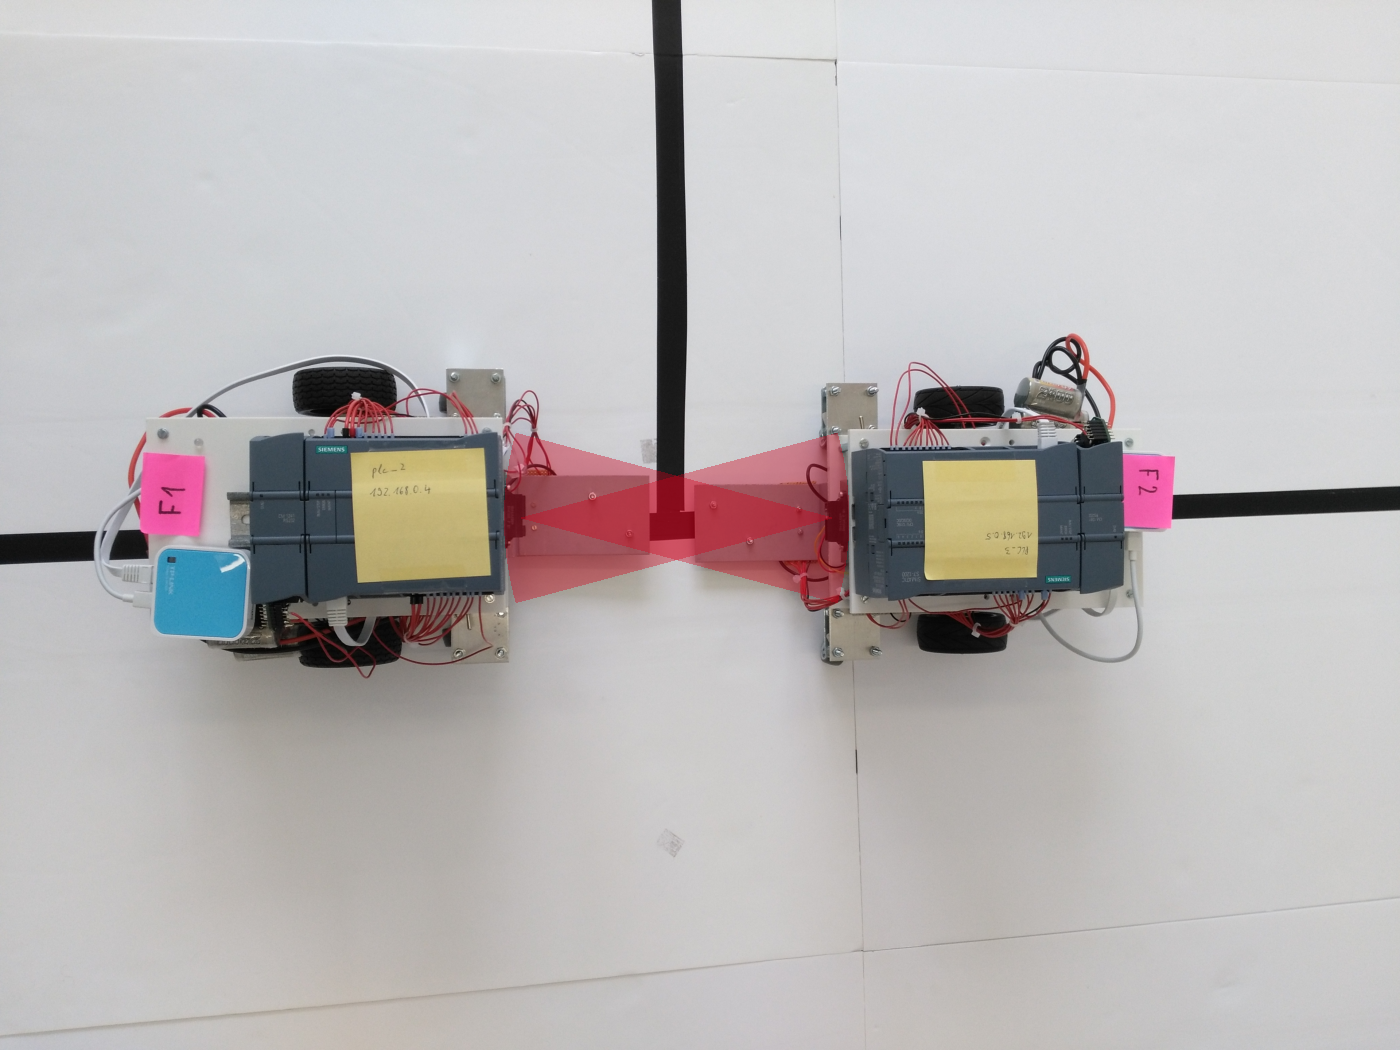
\includegraphics[scale=0.7, trim = 15mm 50mm 25mm 50mm, clip]{/Bilder/FrontalKollisionPDF}
			\vspace{0.2cm}
			\caption{Deadlock bei zu lang eingestellten Kollisionssensoren. Fahrzeuge erkennen sich gegenseitig bevor sie die Kreuzung erreichen.}\label{FronalKollision}
		\end{figure}
		
		Zur Lösung dieses Problems muss entweder den Fahrzeugen eine Priorität beim Einfahren am selben Knoten vergeben werden, damit das niedrigpriore \ac{FTF} die Kreuzung für das hochpriore Fahrzeug freigibt, oder eine solche Annäherung an den gleichen Zielknoten muss algorithmisch verhindert werden. Da im Normalfall eine Reaktion auf andere Fahrzeuge jedoch funktioniert und zum Projektende die Zeit für eine Implementierung und nachfolgende Tests dieser zusätzlichen Funktionen nicht zur Verfügung stand, wurde eine Lösung für dieses Problem bisher noch nicht implementiert.
		\\[4pt]
		Ähnlich zu der soeben beschriebenen Situation kann es passieren, dass zwei Fahrzeuge kollidieren, wenn sie sich zeitnah seitlich im 90°-Winkel an eine Kreuzung annähern. Da die Kollisionssensoren nur Hindernisse vor sich erkennen können, kann es vorkommen, dass sich die Sensorausleger verkeilen, wenn die Fahrzeuge ungefähr zeitgleich in die Kreuzung einfahren. Abbildung \ref{SideKollision} zeigt, wie sich die Fahrzeuge aufgrund der Sensoranordnung gegenseitig nicht erkennen und gleichzeitig versuchen in die Kreuzung einzufahren. Zum Abfangen dieser Situation bedarf es jedoch zusätzlicher Sensoren seitlich am Fahrzeug, die an Kreuzungen quer fahrende Fahrzeuge detektieren können. Ein Umbau der Hardware des \ac{FTF} war jedoch zeitlich nicht mehr realisierbar.
		
		\begin{figure}[h]
			\centering
			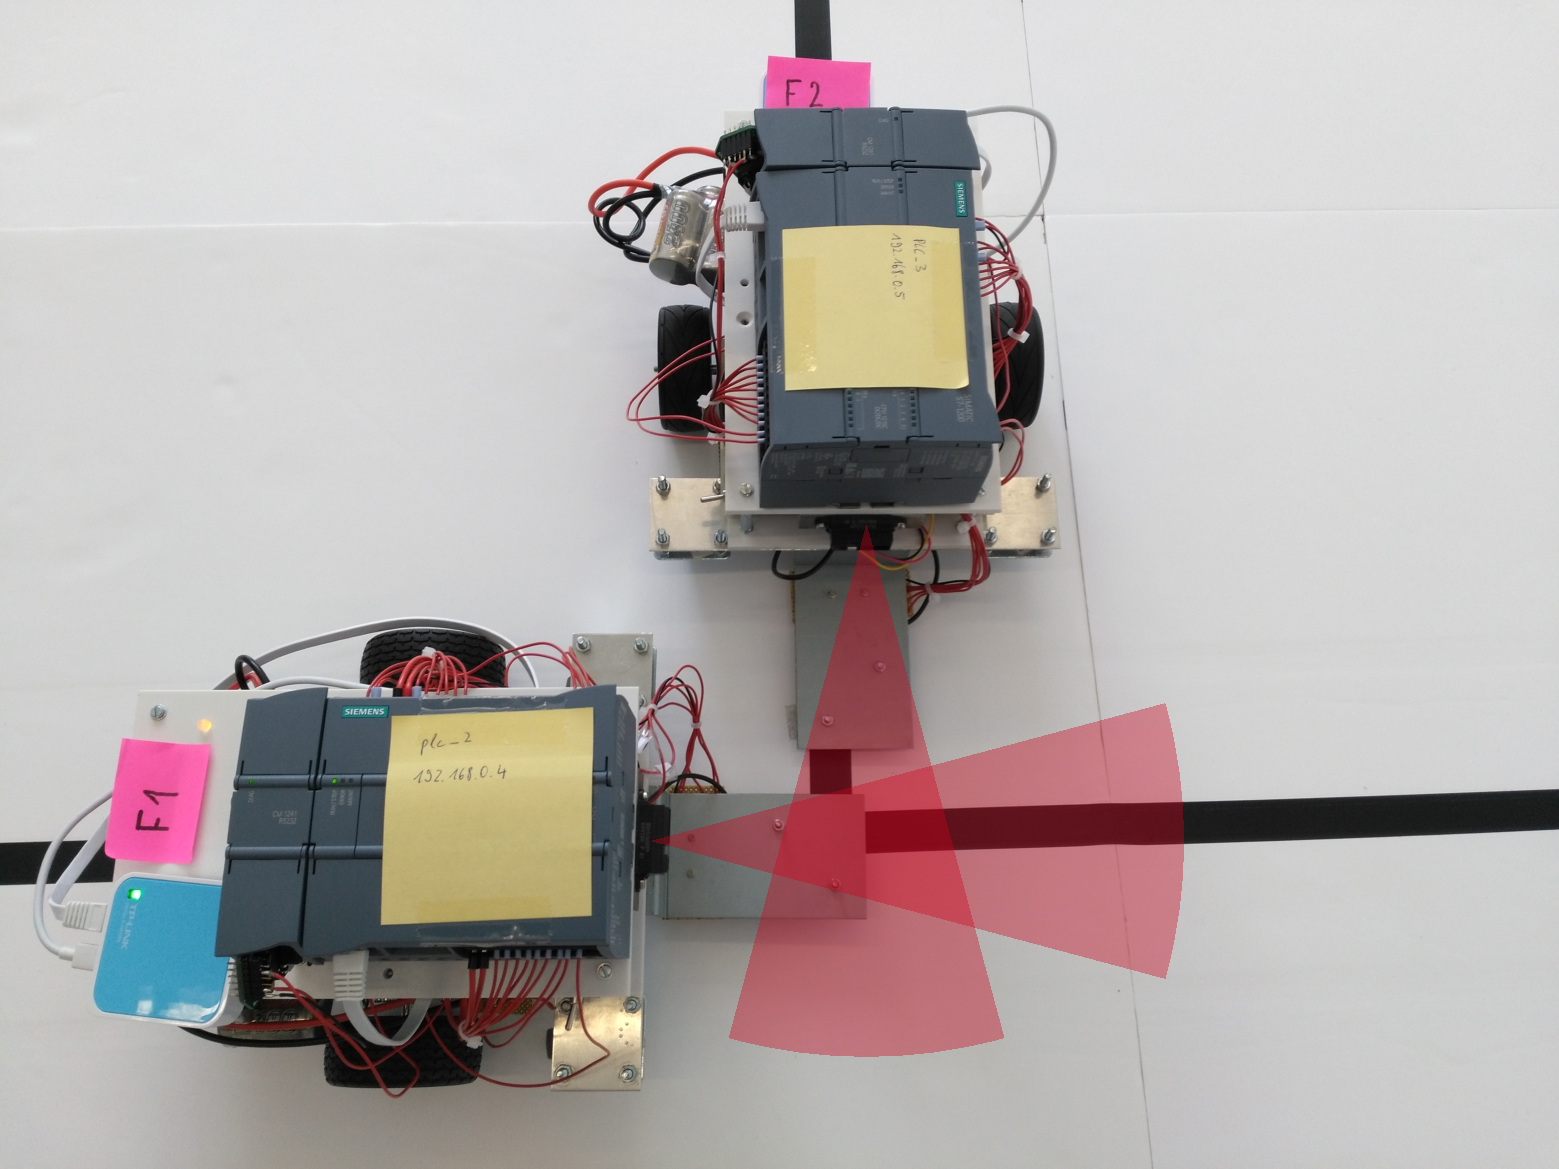
\includegraphics[scale=0.6, trim = 5mm 5mm 55mm 5mm, clip]{/Bilder/SideKollisionPDF}
			\vspace{0.2cm}
			\caption{Situation bei bevorstehender, seitlicher Kollision an einer Kreuzung. Kreuzende Fahrzeuge werden nicht durch den Frontalsensor erkannt.}\label{SideKollision}
		\end{figure}
	
\section{Ausblick über zukünftige Erweiterungen}
	
	Als wichtigster nächster Schritt ist zunächst die Implementierung der in Abschnitt \ref{Probleme_Hardware} beschriebenen Lösungen zur Verhinderung von Kollisionen an Kreuzungen zu erwähnen. Dies verhindert die vereinzelt auftretenden fatalen Fehler, die einen manuellen Eingriff erfordern.\\
	Eine weitere  geplante Anlagenerweiterung ist die Auslagerung der in Abschnitt \ref{Simulation Station} beschriebenen Simulation der Bearbeitungszeit an die jeweiligen Steuerungen der Stationen. Geplant ist hier ein Anmelden des Fahrzeugs an der jeweiligen Bearbeitungsstation und eine Rückmeldung der Station, sobald die Bearbeitung abgeschlossen ist. Dies ermöglicht unterschiedliche Bearbeitungszeiten an unterschiedlichen Maschinen und lässt somit eine bessere Analyse des Werkstückflusses durch die Anlage zu. Es könnte hier zum Beispiel untersucht werden, inwiefern die doppelte Ausführung von Stationen mit langer Bearbeitungszeit einen Einfluss auf die Produktivität der Anlage haben.
	\\[4pt]
	Ähnlich der Auslagerung der Bearbeitungszeit ist auch eine zentrale Zuweisung von Rezepten beim Einfahren in die Anlage in Planung. Dies simuliert die Anbindung an ein der Anlage übergeordnetes Betriebsleitsystem\footnote{englisch: \ac{MES}}, welches zentral bestimmt, welche Art von Produkten benötigt wird und dann bei Bedarf das passende Rezept an einen Werkstückträger in der Anlage zuweist.
	\\[4pt]
	Zudem ist geplant, die Bearbeitungsschritte innerhalb eines Rezeptes variabler zu gestalten. So soll es beispielsweise möglich sein, dass es für ein Werkstück egal ist, in welcher Reihenfolge die  Bearbeitungsschritte 3, 4 oder 5 abgearbeitet werden. Einzige Voraussetzung soll sein, dass alle Schritte ausgeführt wurden bevor Bearbeitungsschritt 6 ausgeführt wird. Dies ermöglicht eine erhöhte Dynamik innerhalb der Anlage, da es in diesem Fall möglich ist, zunächst die Bearbeitungsstation für die Funktionalität 5 als Ziel auszuwählen, wenn zu diesem Zeitpunkt alle Bearbeitungsstationen mit der Funktion 4 bereits belegt sind.
	\\[4pt]
	Eine letzte gewünschte Zusatzanforderung ist die Weiterentwicklung der Visualisierung der Anlage. Diese soll so erweitert werden, dass auf dem Bildschirm ein einzelnes aktives Fahrzeug ausgewählt und teilweise gesteuert werden kann. Somit soll beispielsweise eine Manipulation der Reihenfolge von Bearbeitungsschritten des aktuellen Rezeptes möglich sein, oder die Zuweisung eines komplett neuen Rezeptes. Dies würde ein gewisses Maß an Interaktion bei Vorführungen der Modellanlage bei Kunden ermöglichen.

\section{Zusammenarbeit mit der Entwicklungsabteilung \ac{CT}}

	Parallel zur Entwicklung der Anlage wurde mit der Entwicklungsabteilung der Siemens AG die Grundlage für eine Simulation der realisierten Anlage gelegt. Der Anlagenaufbau sowie Teile der Funktionalität wurden gemeinsam definiert und Use-cases formuliert, die innerhalb einer rechnergestützten Simulation der Anlage mit den Daten des realen Modells verglichen werden können. Zudem kann in bestimmten Zeitintervallen der Zustand der Simulation mit dem wirklichen Anlagenzustand synchronisiert werden. Dies würde es theoretisch ermöglichen, die in Abschnitt \ref{Zeitproblem} erwähnte einstufige Routenvorhersage zu verbessern. Da der Simulation zusätzliche Informationen über alle Fahrzeuge zur Verfügung stehen, welche die Wegfindung aufgrund ihres dezentralen Aufbaus nicht nutzen kann, wäre es denkbar, dass durch Rückmeldung der Simulation an die einzelnen Steuerungen die Wegfindung verbessert werden kann, ohne diese bei Ausfall des zentralen Rechners komplett zu verlieren.
	
\section{Bewertung des Projekts}
	
	Vor Beginn des Projekts war ich zunächst etwas skeptisch, dass sich eine derartig komplexe Funktion wie die Wegfindung auf einem System mit so vielen Beschränkungen wie eine \ac{SPS} überhaupt realisieren lassen würde. Bei der Recherche wurde aber schnell klar, das es grundsätzlich nicht nötig ist, die Wegfindung auf ein PC-System auszulagern, sondern das diese Aufgabe komplett auf einer industriellen Steuerung realisierbar ist. Vor allem die Überwindung von Stolpersteinen bei der Implementierung brachte interessante Herausforderungen, die zu Beginn des Projektes noch gar nicht absehbar waren. Es ist jedoch auch zu sagen, dass die Realisierung einer derartigen Funktion etwas zeitaufwendiger ist als eine vergleichbare Lösung auf einem PC, da auf der PC-Seite oft auf bestehenden Lösungen aufgebaut werden kann. Dies ist bei der Implementierung auf einer \ac{SPS} nicht der Fall. Trotz des Fehlens eines Debuggers und dem damit verbundenen erhöhten Entwurfsaufwands war vor allem die Herausforderung der Aufgabe ein Ansporn, nicht nur ein funktionierendes, sondern auch ein effizientes Wegfindungssystem zu entwickeln. Durch die übergeordnete Aufgabe des Entwurfs einer Modellanlage und die dadurch greifbaren Ergebnisse war das Projekt auch für mich, als eher an der Programmierung interessiertem Menschen, eine interessante Aufgabe. Durch die Zusammenarbeit mit dem Bearbeiter der Fahrzeugsteuerung wurde auch das Arbeiten innerhalb eines Teams mit Eigenverantwortung für die eigenen Themenbereiche gut erprobt und bewältigt.

\section{Zusammenfassung}
	
	Viele Aspekte von Industrie 4.0 werden in den kommenden Jahren immer mehr an Bedeutung gewinnen. Aus diesem Grund ist es für Firmen unabdingbar, ihre Produktion so effizient wie möglich zu gestalten. Im Zuge dessen halten vermehrt Konzepte der IT und der klassischen Informatik Einzug in den Produktionsablauf. Unter diesem Gesichtspunkt ist es interessant zu untersuchen, inwiefern sich diese Konzepte in die Abläufe der Automatisierungstechnik einbinden lassen. Diese Arbeit zeigt, dass es generell möglich ist, selbst komplexere Algorithmen auf industriellen Standardsteuerungen zu realisieren. Durch die Implementierung eines dezentralen Wegfindungsalgorithmus auf Basis des A*-Algorithmus mit exakter Heuristik, wurde auf einer \ac{SPS} der S7-1200er Reihe eine beispielhafte Implementierung erarbeitet. Trotz der Beschränkungen der Steuerungen bezüglich des Speicherplatzes und der Vorhersagbarkeit der Bewegungen anderer Fahrzeuge, lässt sich mittels geeigneter Handhabung der Fahrzeuginformationen verhindern, dass sich die Fahrzeuge in den meisten Fällen gegenseitig behindern. Ganz lässt sich die Wahrscheinlichkeit einer Kollision zum derzeitigen Stand der Anlage noch nicht vermeiden, jedoch wurde der Weg für eine Behebung dieser und anderer Schwachstellen aufgezeigt. Die Routenberechnung ermöglicht es in Verbindung mit dem implementierten Fahrerlosen Transportsystem, Werkstücke anhand verschiedener Rezepturen innerhalb der gleichen Produktionslinie gemeinsam produzieren zu können. Anhand der realisierten Modellanlage lassen sich somit die Industrie 4.0-Konzepte der Dezentralisierung, des autonomen Fahrens sowie der Anlagenskalierbarkeit in geeigneter Form darstellen und für potentielle Kunden vorführen.
	
	
	
	
	%% Beim Anhang gibt es eine Musterdatei, die 
	%% ergänzt werden kann
	%\include{Anhang}
	%\printnomenclature
	
	%% Stichwortverzeichnis ausgeben.
	%% falls nicht notwendig, die folgende Zeile loeschen
	%\printindex
		\pagenumbering{roman}
	
	\chapter{Anhang}
	
	\clearpage
	\addcontentsline{toc}{section}{Literaturverzeichnis}
	\bibliographystyle{ieeetr}
	\bibliography{Sources}
	\clearpage
	\addcontentsline{toc}{section}{Abbildungsverzeichnis}
	\clearpage
	
	
	
	%\printbibliography
	

	
	
\end{document}